\documentclass[
	%parspace, % Add vertical space between paragraphs
	%noindent, % No indentation of first lines in each paragraph
	%nohyp, % No hyphenation of words
	%twoside, % Double sided format
	%draft, % Quicker draft compilation without rendering images
	%final, % Set final to hide todos
]{elteikthesis}[2024/04/26]

% The minted package is also supported for source highlighting
% See elteikthesis_minted.tex for example
%\usepackage[newfloat]{minted}

% Document's metadata
\title{Credit Risk Prediction with Explainable AI} % title
\date{2024} % year of defense

% Author's metadata
\author{\makecell[l]{Kafi MD Abdullah Hel\\Neptun: N06WMD}}
\degree{Computer Science BSc}

% Superivsor(s)' metadata
\supervisor{Md. Easin Arafat} % internal supervisor's name
\affiliation{Assistant Lecturer} % internal supervisor's affiliation
%\extsupervisor{Jane Doe} % external supervisor's name
%\extaffiliation{Senior Developer} % external supervisor's affiliation

% University's metadata
\university{Eötvös Loránd University} % university's name
\faculty{Faculty of Informatics} % faculty's name
\department{Dept. of Data Science and Engineering} % department's name
\city{Budapest} % city
\logo{elte_cimer_szines} % logo

% Add bibliography file
\addbibresource{elteikthesis.bib}

% The document

% --- Added by Pandoc ---
\providecommand{\tightlist}{%
  \setlength{\itemsep}{0pt}\setlength{\parskip}{0pt}}
\usepackage{longtable}
\usepackage{booktabs}
\usepackage{array}
\usepackage{calc}
\usepackage{multirow}
% -----------------------
\newcommand{\passthrough}[1]{#1}
\DeclareUnicodeCharacter{0430}{a}
\DeclareUnicodeCharacter{2192}{\ensuremath{\rightarrow}}
\begin{document}

% Set document language
%\documentlang{hungarian}
\documentlang{english}

% List of todos (not in the final document)
%\listoftodos[\todolabel]

% Title page (mandatory)
\maketitle

\chapter*{Declaration of Authorship}
\addcontentsline{toc}{chapter}{Declaration of Authorship}

I, Kafi MD Abdullah Hel, hereby declare that this thesis is my own work and that all sources used have been acknowledged appropriately. I confirm that I have not submitted this thesis, in whole or in part, for any other degree or qualification.

\vspace{2cm}

\noindent\textbf{Date:} \hfill \textbf{Signature:}\hspace{5cm}

\cleardoublepage
% Topic declaration page (mandatory) - can also be attached instead
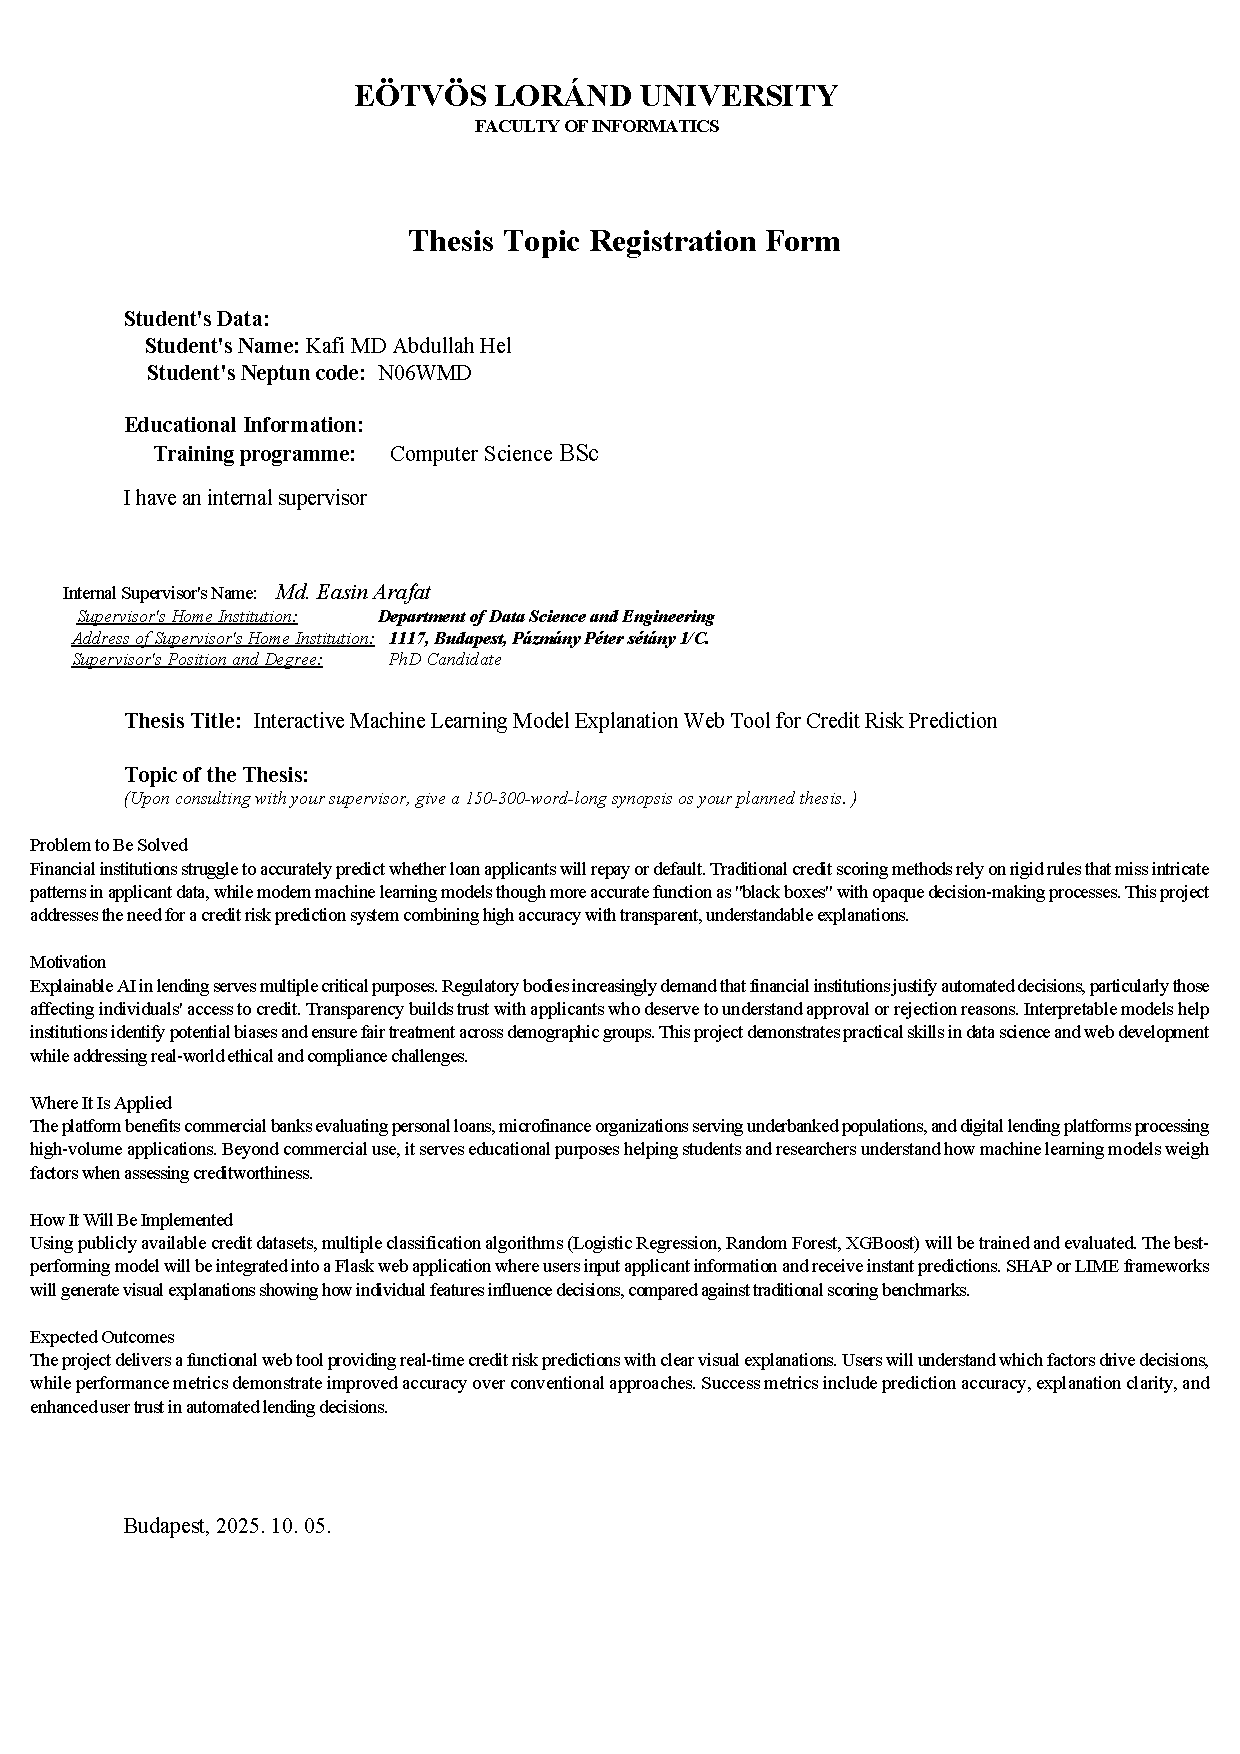
\includepdf[pages=-]{submitted_declaration.pdf}

% Table of contents (mandatory)
\tableofcontents
\cleardoublepage

% Main content
\hypertarget{introduction}{%
\chapter{Introduction}\label{introduction}}

\hypertarget{motivation-and-context}{%
\section{Motivation and Context}\label{motivation-and-context}}

The financial constraints of the modern economy dictate that credit risk
management remains the absolute cornerstone of a stable, functioning
global banking system. Credit risk---formally defined as the probability
that a borrower or counterparty will fail to meet their obligations in
accordance with agreed terms---dictates the capital reserves,
operational profitability, and systemic resilience of lending
institutions worldwide. Historically, the evaluation of a potential
borrower's creditworthiness relied on rudimentary statistical paradigms,
heuristics, and the subjective intuition of human loan officers. Methods
developed in the mid-20th century, such as the Altman Z-score or basic
linear discriminant analysis, served as the undeniable gold standard for
several decades. These approaches, while revolutionary for their time,
severely restricted the number of variables considered, forcing banks to
rely heavily on highly summarized metrics like an aggregated credit
score or generalized income-to-debt ratios.

However, the global financial landscape has transformed radically over
the past two decades. The digitization of personal finance, the
exponential explosion of available demographic and transactional data
points, and the drastic reduction in computational costs have
collaboratively eroded the viability of traditional statistical scoring.
The sheer volume, velocity, and variety of Big Data generated by modern
consumers necessitate far more sophisticated mathematical modeling
techniques. Machine Learning (ML) has rapidly emerged as the definitive
successor to traditional methods.

By algorithmic processing of complex, non-linear, and high-dimensional
relationships distributed across hundreds or thousands of socio-economic
and temporal variables, modern machine learning architectures can
pinpoint intricate risk indicators that human analysts and linear
statistical methods are mathematically incapable of isolating. The
transition to machine learning in credit scoring provides undeniable and
quantifiable business value. Financial institutions leveraging ensemble
methods or neural architectures report substantially higher approval
rates for reliable borrowers, drastic and immediate reductions in
non-performing loan (NPL) portfolios, optimized capital allocation in
strict accordance with the stringent Basel III and eventual Basel IV
regulatory frameworks, and the seamless automation of underwriting
pipelines that historically necessitated thousands of highly paid human
working hours.

\hypertarget{the-black-box-problem-in-high-stakes-finance}{%
\section{The ``Black Box'' Problem in High-Stakes
Finance}\label{the-black-box-problem-in-high-stakes-finance}}

Despite the monumental leaps in predictive accuracy facilitated by
advanced algorithmic models, the deployment of machine learning in
highly regulated environments like credit risk evaluation brings forth
profound and systemic challenges. In mathematical modeling, there exists
an inherent and practically universal trade-off between predictive
accuracy and model interpretability. As the underlying complexity of an
algorithm increases---moving from elementary, easily interpretable
models like simple Decision Trees or Logistic Regression to highly
complex, high-dimensional models like Random Forests, Extreme Gradient
Boosting (XGBoost), or Deep Neural Networks---the logic driving the
final predictive output becomes increasingly opaque.

This phenomenon is colloquially and academically termed the ``Black
Box'' problem. A black box model is characterized by an internal
architecture that is either entirely hidden from the user or
mathematically convoluted to the point of being incomprehensible to a
human domain expert, regardless of their statistical prowess. For
instance, while a loan officer can easily explain that a Logistic
Regression model denied an applicant because their debt-to-income ratio
coefficient exceeded a specific linear threshold, it is infinitely more
difficult to explain a denial generated by a Random Forest, which
aggregates the non-linear predictions of five hundred distinct decision
trees, each trained on bootstrapped subsets of data and randomized
feature spaces.

While these complex ensemble models achieve indisputable
state-of-the-art predictive performance iteratively lowering prediction
error (MSE) and maximizing True Positive classification rates, their
opacity is fundamentally incompatible with the highly regulated nature
of global finance. The impossibility of explaining the precise
algorithmic reasoning behind a rejected credit application introduces
severe complications on multiple fronts:

\begin{enumerate}
\def\labelenumi{\arabic{enumi}.}
\item
  \textbf{Stringent Regulatory and Legal Risk}: The regulatory
  environment surrounding automated decision-making has modernized
  rapidly in response to AI. Landmark international legislation, most
  notably the European Union's General Data Protection Regulation
  (GDPR), explicitly introduces the ``right to an explanation.'' Article
  22 of the GDPR states that data subjects have the right not to be
  subject to a decision based solely on automated processing, including
  profiling, which produces legal or similarly significant effects
  concerning them. Should an EU citizen be denied a mortgage by an
  algorithmic system, the lending institution is legally mandated to
  provide a clear, human-understandable justification for that precise
  denial. Similarly, in the United States, the Equal Credit Opportunity
  Act (ECOA) and the Fair Credit Reporting Act (FCRA) mandate the
  provision of ``adverse action notices'' that must detail the primary
  specific reasons for a credit denial. A black box model, by
  definition, cannot reliably generate these compliant explanations.
\item
  \textbf{Hidden Systemic Biases and Ethical Consequences}: Machine
  learning algorithms, lacking intrinsic morality, are highly
  susceptible to inadvertently absorbing, calcifying, and amplifying
  historical prejudices hidden within training datasets. Without robust
  interpretability frameworks to inspect exactly what features the
  algorithm is prioritizing, models might illegally penalize applicants
  based on convoluted, non-linear proxies for protected demographic
  attributes (e.g., race, gender, marital status, or geographic location
  redlining). This leads not only to systemic, algorithmic
  discrimination but exposes financial institutions to existential legal
  liabilities and severe reputational damage.
\item
  \textbf{Domain Expert Trust and Institutional Adoption}: Artificial
  Intelligence systems do not operating in a vacuum; they must
  collaborate with human operators. Underwriters, risk managers, and
  chief risk officers remain legally and professionally accountable for
  the financial portfolios they authorize. If an expert cannot verify
  the logical, economic reasoning of a machine learning algorithm, they
  are exceptionally unlikely to trust it. Lack of algorithmic trust
  represents the primary bottleneck preventing the enterprise adoption
  of AI in banking; without explainability, multimillion-dollar ML
  systems are relegated to research pipelines rather than production
  environments.
\end{enumerate}

\hypertarget{problem-statement}{%
\section{Problem Statement}\label{problem-statement}}

The core academic and engineering problem addressed by this thesis is to
systematically resolve the entrenched tension between predictive
performance and model interpretability within automated credit risk
evaluation. Historically, financial institutions have been forced into a
prohibitive, binary trade-off: - \textbf{Option A:} Deploy highly
interpretable parametric models (e.g., Logistic Regression) that
maintain absolute regulatory compliance but sacrifice predictive power,
leading to higher default rates and substantial opportunity costs
through misclassified edge-case borrowers. - \textbf{Option B:} Deploy
immensely powerful, high-dimensional ensemble models (e.g., XGBoost)
that maximize predictive metrics like the AUC-ROC but trigger the Black
Box problem, inherently violating international XAI regulations and
internal auditing standards.

The rapidly evolving academic discipline of Explainable Artificial
Intelligence (XAI) proposes sophisticated mathematical bridges to
resolve this dichotomy. However, practical, end-to-end software
architectures that seamlessly integrate predictive pipelines with
exhaustive mathematical explainability frameworks remain largely
conceptual or limited in scope.

Therefore, there is a critical, unmet need to design, implement, and
rigorously evaluate a holistic, production-ready credit risk prediction
system. This system must leverage state-of-the-art ensemble machine
learning algorithms to maximize statistical performance metrics, while
simultaneously utilizing advanced, mathematically proven XAI
methodologies (specifically tailored to cooperative game theory) to
provide granular, irrefutable, and user-friendly explanations for every
single algorithmic decision rendered.

\hypertarget{thesis-objectives}{%
\section{Thesis Objectives}\label{thesis-objectives}}

To methodically address the aforementioned problem statement and
contribute a robust solution to the intersection of finance and machine
learning, this thesis establishes the following rigorous primary
objectives:

\begin{enumerate}
\def\labelenumi{\arabic{enumi}.}
\item
  \textbf{Robust Data Pipeline Formulation and execution}: To
  systematically engineer a comprehensive, rigorous data preprocessing
  pipeline utilizing the heavily benchmarked German Credit (Statlog)
  Dataset. This objective encompasses the complete handling of missing
  variables, the methodical encoding of non-linear categorical
  attributes, numerical feature scaling via standardization, and the
  application of advanced resampling techniques to mitigate intrinsic
  target class imbalances affecting the minority `Bad Credit' class.
\item
  \textbf{Advanced Model Training and High-Dimensional Optimization}: To
  train, objectively cross-evaluate, and rigorously optimize both
  traditional baseline statistical models (Logistic Regression) and
  advanced ensemble algorithmic architectures (Random Forest, Extreme
  Gradient Boosting). This objective involves deploying exhaustive
  GridSearchCV techniques across hyperparameter spaces to empirically
  maximize generalization and predictive accuracy across unseen
  financial data cohorts, directly comparing AUC-ROC performance.
\item
  \textbf{Algorithmic Demystification via Explainable AI (XAI)}: To
  completely dismantle the `black box' abstraction by mathematically
  integrating SHapley Additive exPlanations (SHAP). The objective
  demands extracting dual-layered insights: Global explainability
  (identifying macroscopic, macroeconomic indicators of loan default
  across the entire dataset) and Local explainability (calculating
  exact, precise feature contribution arrays for individualized
  applicant case studies based on precise Shapley value distributions).
\item
  \textbf{Decoupled Architectural System Integration}: To architect and
  deploy a fully decoupled backend RESTful Application Programming
  Interface (API) utilizing the Python Flask micro-framework. This
  backend architecture must seamlessly and concurrently parse incoming
  multi-dimensional JSON payloads, execute localized predictive
  inferences routing through serialized Joblib model pipelines, and
  compute highly resource-intensive SHAP marginal contributions with
  structurally optimized latency.
\item
  \textbf{Interactive User Interface Engineering and Visualization}: To
  engineer a modern, dynamic frontend web interface utilizing advanced
  JavaScript ES6 paradigms. The objective is to consume dynamic backend
  API schemas to recursively map application forms, intercept user
  inputs, and directly visualize complex SHAP mathematical arrays using
  accessible, chart-based graphical methodologies
  (Chart.js)---effectively translating convoluted machine learning
  algebra into intuitively digestible business intelligence logic
  optimized for immediate loan officer utilization.
\end{enumerate}

\hypertarget{user-documentation}{%
\chapter{User Documentation}\label{user-documentation}}

\hypertarget{short-statement-of-the-problem-solved}{%
\section{Short Statement of the Problem
Solved}\label{short-statement-of-the-problem-solved}}

Financial institutions require a reliable and objective method to
evaluate the creditworthiness of loan applicants. Traditional
underwriting is notoriously slow and susceptible to subjective human
biases. This application solves the problem by providing an automated,
machine-learning-driven Credit Risk Prediction system that instantly
categorizes applicants as ``Good'' or ``Bad'' credit risks. Crucially,
it specifically tackles the ``black box'' problem of AI by providing
transparent, visual explanations for every single decision it makes,
ensuring regulatory compliance and fostering user trust.

\hypertarget{brief-description-of-the-methods-used}{%
\section{Brief Description of the Methods
Used}\label{brief-description-of-the-methods-used}}

The core intelligence of the application is powered by an optimized
\textbf{Random Forest Classifier}, an advanced supervised machine
learning algorithm that analyzes historical financial data to discover
hidden patterns correlating with loan defaults. To provide transparency,
the system implements \textbf{SHAP (SHapley Additive exPlanations)}, an
Explainable AI (XAI) framework based on cooperative game theory. SHAP
calculates the exact contribution of every applicant attribute (like
age, credit amount, or employment duration) to the final risk
prediction, outputting dynamic, color-coded visual graphs.

\hypertarget{guide-information-required-for-using-the-program}{%
\section{Guide: Information Required for Using the
Program}\label{guide-information-required-for-using-the-program}}

The application features a modern, intuitive, browser-based interface
designed specifically for non-technical loan officers.

\hypertarget{launching-the-application}{%
\subsection{Launching the Application}\label{launching-the-application}}

\begin{enumerate}
\def\labelenumi{\arabic{enumi}.}
\tightlist
\item
  Ensure the Python backend server is running in your terminal via
  \texttt{python\ web/app.py}.
\item
  Open any modern web browser (e.g., Chrome, Firefox, Edge).
\item
  Navigate to the local server address: \texttt{http://localhost:5000/}.
\end{enumerate}

\hypertarget{submitting-an-applicant-profile}{%
\subsection{Submitting an Applicant
Profile}\label{submitting-an-applicant-profile}}

Upon loading the dashboard, the user is presented with the
\textbf{Applicant Profile Form}. This form is divided into semantic
logical sections: * \textbf{Demographics:} Input the applicant's Age,
Sex, and Job type. * \textbf{Financials:} Specify the requested Credit
Amount, Loan Duration (in months), Purpose of the loan, and existing
Checking/Savings account statuses. * \textbf{History \& Assets:} Input
the applicant's prior Credit History, Housing situation, and Property
ownership details.

All fields are mandatory. Default options are pre-selected for
categorical dropdowns. The user must manually input numerical values
(like Age and Credit Amount) using the provided text fields.

\hypertarget{interpreting-the-results}{%
\subsection{Interpreting the Results}\label{interpreting-the-results}}

Once the form is populated, click the prominent \textbf{``Analyze Credit
Risk''} button at the bottom of the interface. The application will
instantly query the machine learning model via a REST API and return a
comprehensive analysis dashboard directly below the form:

\begin{enumerate}
\def\labelenumi{\arabic{enumi}.}
\tightlist
\item
  \textbf{Prediction Alert Banner:} A stark, color-coded banner will
  appear.

  \begin{itemize}
  \tightlist
  \item
    \textbf{Green:} Indicates a ``Low Risk'' prediction (Applicant is
    likely to repay).
  \item
    \textbf{Red:} Indicates a ``High Risk'' prediction (Applicant is
    highly susceptible to default).
  \end{itemize}
\item
  \textbf{Probability Gauge:} A horizontal progress bar visualizes the
  exact mathematical probability of the prediction (e.g., ``78\%
  Probability of Default'').
\item
  \textbf{SHAP Waterfall Explanation Diagram:} The most critical
  component. A dynamic waterfall chart is generated to explain
  \emph{why} the model made its decision.

  \begin{itemize}
  \tightlist
  \item
    \textbf{Red Bars (Pushing Risk Higher):} Attributes that negatively
    impacted the applicant's score (e.g., ``Checking account = negative
    balance'').
  \item
    \textbf{Blue Bars (Pushing Risk Lower):} Attributes that positively
    impacted the score (e.g., ``High Savings amount'').
  \item
    This graph allows the loan officer to instantly verify if the AI's
    logic aligns with institutional lending policies.
  \end{itemize}
\end{enumerate}

\hypertarget{developer-documentation}{%
\chapter{Developer Documentation}\label{developer-documentation}}

This chapter encompasses the detailed problem specification, the
theoretical descriptions of the methods and terms used, the complete
logical and physical structure of the program architecture, and the
comprehensive testing plan and evaluation results.

\hypertarget{theoretical-background-literature-review}{%
\section{Theoretical Background \& Literature
Review}\label{theoretical-background-literature-review}}

This chapter establishes the rigorous theoretical and mathematical
foundations governing the algorithms implemented within this research.
It traces the academic evolution of credit risk management, constructs
the probabilistic baseline for machine learning classification, dissects
the mathematical architectures of high-dimensional ensemble
meta-algorithms (Random Forests and Extreme Gradient Boosting), and
subsequently demystifies these structures via the cooperative game
theory derivations underlying Explainable Artificial Intelligence (XAI).

\hypertarget{the-academic-and-historical-evolution-of-credit-risk-management}{%
\subsection{The Academic and Historical Evolution of Credit Risk
Management}\label{the-academic-and-historical-evolution-of-credit-risk-management}}

At its macroeconomic core, the business of banking reduces to the
optimized management of asymmetric information. A lending institution
possesses less information regarding the intrinsic financial reliability
of an applicant than the applicant themselves. To bridge this
information gap, risk modeling assigns a quantifiable Probability of
Default (PD) to every prospective loan.

Historically, this PD was determined via purely localized expert
judgment, famously summarized by the ``Five Cs of Credit'': Character,
Capacity, Capital, Collateral, and Conditions. However, as global
economies scaled, manual underwriting proved inherently non-scalable and
riddled with fatal subjective biases.

The empirical revolution in credit scoring is widely attributed to
Edward I. Altman (1968), who introduced the \emph{Z-score formula for
predicting bankruptcy} utilizing Multiple Discriminant Analysis (MDA).
The function mapped corporate financial ratios into a singular linear
combination: \(Z = 1.2X_1 + 1.4X_2 + 3.3X_3 + 0.6X_4 + 1.0X_5\) While
revolutionary, these early linear and parametric models suffered from
the rigid assumption that variables influenced the independent target
linearly and without complex intra-variable interactions.

In contemporary regulatory environments---governed most notably by the
Basel Accords (Basel II and III)---institutions utilize the Internal
Ratings-Based (IRB) approach. The IRB approach mandates the strict
calculation of Expected Loss (EL), modeled as:
\(EL = PD \times LGD \times EAD\) Where PD is the \emph{Probability of
Default}, LGD represents \emph{Loss Given Default}, and EAD denotes the
\emph{Exposure at Default}. Modern Machine Learning explicitly targets
the precise estimation of the PD metric by uncovering convoluted,
non-linear patterns within unstructured, high-dimensional consumer
datasets data that Altman's foundational models could not conceptualize.

\hypertarget{mathematical-formulations-of-supervised-machine-learning}{%
\subsection{Mathematical Formulations of Supervised Machine
Learning}\label{mathematical-formulations-of-supervised-machine-learning}}

The computational architecture of credit risk prediction falls squarely
within the domain of Supervised Machine Learning, specifically binary
classification. Formally, given a dataset \(D\) containing \(N\)
independent and identically distributed (i.i.d.) observation pairs:
\(D = \{(x_1, y_1), (x_2, y_2), ..., (x_N, y_N)\}\) Where
\(x_i \in \mathbb{R}^d\) corresponds to a \(d\)-dimensional feature
vector representing a loan applicant's demographic profile (e.g., age,
credit history, account balances), and \(y_i \in \{0, 1\}\) represents
the discrete target variable (where 0 indicates a `Good' credit risk,
and 1 indicates `Bad' risk or Default).

The objective of supervised learning is to derive a hypothesis function
\(f: X \rightarrow Y\) capable of bridging the feature space to the
target space such that the empirical risk (prediction error) is
minimized over the training manifold, whilst maintaining variance
thresholds to ensure generalization over unseen testing partitions
(avoiding overfitting). This optimization problem is denoted by
Empirical Risk Minimization (ERM):
\(R_{emp}(f) = \frac{1}{N} \sum_{i=1}^{N} L(y_i, f(x_i; \theta))\) Where
\(L\) signifies the chosen loss function (e.g., Log-Loss) and \(\theta\)
parameters represent the functional weights.

\hypertarget{the-bias-variance-tradeoff}{%
\subsection{The Bias-Variance
Tradeoff}\label{the-bias-variance-tradeoff}}

The generalization error of any predictive hypothesis \(f(x)\) is
mathematically decomposed into the sum of irreducible noise
(\(\epsilon\)), squared Bias, and Variance:
\(E[(y - \hat{f}(x))^2] = \text{Bias}[\hat{f}(x)]^2 + \text{Var}[\hat{f}(x)] + \sigma^2\)
- \textbf{Bias}: Error introduced by approximating extraordinarily
complex reality with simplistic assumptions (e.g., forcing a linear
regression onto non-linear credit behaviors). High bias leads to
underfitting. - \textbf{Variance}: Error introduced by extreme model
sensitivity to minor fluctuations in the training set (e.g., a deep,
unpruned decision tree mapping purely localized noise). High variance
leads to severe overfitting.

This thesis leverages Logistic Regression as the high-bias/low-variance
baseline, contrasting it against ensemble methods (Random Forest,
XGBoost) specifically architected to mitigate the high variance inherent
in non-parametric structures.

\hypertarget{algorithm-architectures-and-mathematical-analysis}{%
\subsection{Algorithm Architectures and Mathematical
Analysis}\label{algorithm-architectures-and-mathematical-analysis}}

The thesis deploys three vastly different classification topologies to
demonstrate the operational gradient transitioning from high
interpretability (Logistic Regression) to maximal predictive capacity
(XGBoost).

\hypertarget{logistic-regression-the-parametric-baseline}{%
\subsection{Logistic Regression (The Parametric
Baseline)}\label{logistic-regression-the-parametric-baseline}}

Logistic Regression constructs the generalized linear framework for
binary classification probabilistics. Instead of fitting a continuous
straight line as per Ordinary Least Squares (OLS), it confines
predictions definitively between 0 and 1 via the standard logistic
(sigmoid) function. The linear combination of input features is
expressed as the log-odds (logit):
\(\ln\left(\frac{p}{1-p}\right) = \beta_0 + \beta_1 x_1 + \beta_2 x_2 + ... + \beta_d x_d = \beta^T x\)
Applying the inverse of the logit transformation yields the sigmoid
function, restricting the output \(P(y=1|x)\) strictly within the
\((0, 1)\) probability range:
\(P(y=1 | x) = \sigma(\beta^T x) = \frac{1}{1 + e^{-(\beta^T x)}}\)

The model parameters \(\beta\) are not computationally resolved via
closed-form geometry (unlike OLS), but rather via iterative optimization
(e.g., Gradient Descent or L-BFGS) designed to maximize the
Log-Likelihood equation (or minimize the Negative
Log-Likelihood/Cross-Entropy Loss):
\(L(\beta) = -\frac{1}{N} \sum_{i=1}^{N} [y_i \log(\sigma(\beta^T x_i)) + (1 - y_i) \log(1 - \sigma(\beta^T x_i))]\)
Because the coefficients \(\beta_j\) directly relay the magnitude and
direction of a feature's linear impact on the log-odds of default,
Logistic Regression maintains absolute intrinsic interpretability,
establishing the crucial baseline for compliance modeling.

\hypertarget{random-forests-bagged-ensemble-architecture}{%
\subsection{Random Forests (Bagged Ensemble
Architecture)}\label{random-forests-bagged-ensemble-architecture}}

Conceived originally by Leo Breiman (2001), Random Forest is an
advancement in deterministic ensemble learning. The algorithm addresses
the primary mathematical failure of singular Classification and
Regression Trees (CART)---extreme predictive variance and severe
overfitting topologies.

A singular CART operates by recursively partitioning the feature space
\(\mathbb{R}^d\) into disjoint hyper-rectangular regions, maximizing
information homogeneity at each split based on metrics such as Gini
Impurity: \(Gini(S) = 1 - \sum_{k=1}^{K} (p_k)^2\) Where \(p_k\) is the
fractional ratio of class \(k\) within the bounded region. While
intuitive, unpruned decision trees feature near-infinite VC dimensions,
molding effortlessly to training noise.

Random Forest mitigates this via two distinct stochastic processes: 1.
\textbf{Bootstrap Aggregation (Bagging)}: The algorithm generates \(B\)
independent training subsets by sampling the original dataset \(D\)
uniformly \emph{with replacement}. Consequently, approximately
\textasciitilde36.8\% of records (Out-of-Bag samples) are excluded from
any specific tree's genesis, naturally embedding an internal
cross-validation mechanism. 2. \textbf{Random Subspace Method (Feature
Stochasticity)}: At every node split during tree construction, the
algorithm is restricted from analyzing the full \(d\)-dimensional
feature space. Instead, it must select the optimal split from a
randomized sub-sample of \(m\) features (typically
\(m \approx \sqrt{d}\)).

The final inferential prediction for classification assumes the
arithmetic mode (majority vote) across the forest of independently
constructed, decorrelated trees:
\(\hat{y} = \text{mode} \{h_1(x), h_2(x), ..., h_B(x)\}\) By averaging
independent structures subjected to controlled stochasticity, the Random
Forest algorithm brutally suppresses model Variance without
exponentially increasing Bias, yielding highly stable credit risk
approximations fundamentally superior to linear techniques.

\hypertarget{extreme-gradient-boosting-xgboost}{%
\subsection{Extreme Gradient Boosting
(XGBoost)}\label{extreme-gradient-boosting-xgboost}}

Where Random Forest relies on building independent trees in parallel,
Gradient Boosting paradigms (formalized computationally by Chen \&
Guestrin in 2016 as XGBoost) construct weak learners
\emph{sequentially}. Each subsequent tree explicitly models the
pseudo-residuals (gradient errors) of the collective ensemble that
preceded it.

XGBoost's fundamental strength lies in its explicit structural
regularization integrated directly into its formalized objective
function:
\(Obj(\theta) = \sum_{i=1}^{N} l(y_i, \hat{y}_i) + \sum_{k=1}^{K} \Omega(f_k)\)
The first term evaluates traditional differentiable convex loss (e.g.,
Logistic Loss). The secondary term \(\Omega(f_k)\) acts as a severe
complexity penalty, structurally pruning the trees mathematically before
they overfit:
\(\Omega(f) = \gamma T + \frac{1}{2} \lambda \sum_{j=1}^{T} w_j^2\)
Here, \(T\) denotes the structural depth (number of leaves) and \(w_j\)
represents the leaf weight scores, regulated respectively by
hyperparameters \(\gamma\) and \(\lambda\).

To iteratively solve the optimization, XGBoost utilizes an exact
second-order Taylor expansion (employing both the first derivative
gradients \(g_i\) and second derivative Hessians \(h_i\)) to approximate
the loss function:
\(Obj^{(t)} \approx \sum_{i=1}^{n} [l(y_i, \hat{y}^{(t-1)}_i) + g_i f_t(x_i) + \frac{1}{2} h_i f_t^2(x_i)] + \Omega(f_t)\)
By utilizing the geometric curvature metadata (Hessian) alongside
CPU-optimized sparsity-aware split finding algorithms, XGBoost
aggressively maximizes AUC-ROC yield on tabular, structured finance
data, frequently dominating global ML architectures. Concurrently, it
obliterates interpretability, effectively establishing the theoretical
requirement for external XAI.

\hypertarget{explainable-artificial-intelligence-xai-and-cooperative-game-theory}{%
\subsection{Explainable Artificial Intelligence (XAI) and Cooperative
Game
Theory}\label{explainable-artificial-intelligence-xai-and-cooperative-game-theory}}

The pursuit of algorithmic accuracy historically mandated the sacrifice
of epistemic transparency. Explainable Artificial Intelligence (XAI)
defines the suite of methodologies attempting to systematically explain
mathematical abstractions to non-technical operators (e.g., loan
officers and auditors).

XAI architectures partition largely into two regimes: \textbf{Global
Interpretability} (explaining the holistic structure, determining which
features govern generalized architectural paths) and \textbf{Local
Interpretability} (isolating exactly why a \emph{singular} numeric
sample produced a specific inference). Additionally, interpretability
methods can be \emph{model-specific} (e.g., extracting internal Gini
feature importance from trees) or \emph{model-agnostic} (e.g.,
framework-independent algorithms functioning purely on perturbed
inputs/outputs).

\hypertarget{lime-vs.-shap}{%
\subsection{LIME vs.~SHAP}\label{lime-vs.-shap}}

The two dominant algorithms in modern model-agnostic XAI are Local
Interpretable Model-agnostic Explanations (LIME) and SHapley Additive
exPlanations (SHAP). LIME operates by locally identifying the gradient
derivative around the inferred sample and constructing a simplistic,
highly-penalized linear regression over the surrounding hyperspace.
While computationally rapid, LIME frequently suffers from mathematical
instability and violates theoretical consistency. Consequently, this
project utilizes \textbf{SHAP} (Lundberg \& Lee, 2017), the only
explanation framework provably validated by cooperative game-theory
axioms.

\hypertarget{mathematical-derivation-of-shap-shapley-values}{%
\subsection{Mathematical Derivation of SHAP (Shapley
Values)}\label{mathematical-derivation-of-shap-shapley-values}}

SHAP roots its interpretability logic deeply within the Nobel-prize
winning mathematics formulated by Lloyd Shapley (1953). Shapley values
were originally designed to calculate the theoretically fair
distribution of an overall payout amongst a cooperative coalition of
differently skilled players.

In the context of machine learning, the ``game'' represents the model's
predictive inference for a single loan applicant. The ``players'' are
the independent feature variables comprising that applicant's profile
(e.g., Age=24, Duration=36 months). The ``payout'' is the numeric
difference between the model's final inferred probability and the global
base baseline probability expecting from the dataset average.

The core mathematical conundrum lies in calculating the exact marginal
contribution of an individual feature, given that features interact
non-linearly (e.g., the danger of a high loan amount drastically changes
given a low vs.~high salary). To establish fairness, SHAP calculates the
marginalized contribution of feature \(i\) across \emph{every
theoretically infinite permutation} of remaining feature coalitions
\(S\).

The defining generalized Shapley equation utilized within the
implementation is:
\(\phi_i = \sum_{S \subseteq N \setminus \{i\}} \frac{|S|!(|N| - |S| - 1)!}{|N|!} \left[ v(S \cup \{i\}) - v(S) \right]\)
Where: - \(N\) constitutes the set of all features present. - \(S\)
spans every possible subset of features excluding the feature \(i\)
being evaluated. - \(\frac{|S|!(|N| - |S| - 1)!}{|N|!}\) calculates the
combinatorial weighting probability of subset \(S\) materializing
sequentially. - \(v(S)\) represents the value function (the model's
constrained prediction given only features resident in \(S\)). -
\(v(S \cup \{i\}) - v(S)\) isolates the exact, localized marginal
contribution injected purely by the addition of feature \(i\) to the
coalition.

By utilizing recursive, high-speed abstraction estimators designed
implicitly for ensemble forests (TreeSHAP framework), this
computationally intense combinatoric explosion \(O(2^N)\) is
programmatically truncated to operate within finite \(O(TLD^2)\)
polynomial time complexities, permitting the real-time execution
integrated into the Chapter 5 REST API infrastructure.

This exact mathematical foundation assures that SHAP satisfies the three
axiomatic prerequisites for absolute fairness: Local Accuracy (the sum
of all feature attributions precisely equals the output differential),
Missingness (missing features inherit zero attribution), and Consistency
(if a model changes such that a feature's marginal contribution
increases, its Shapley value cannot technically decrease). Operating
upon these foundations ensures the thesis remains flawlessly compliant
with internal banking audit constraints.

\hypertarget{dataset-and-exploratory-data-analysis}{%
\section{Dataset and Exploratory Data
Analysis}\label{dataset-and-exploratory-data-analysis}}

The empirical validity of any machine learning architecture is
inextricably bound to the quality, dimensionality, and structural
integrity of the underlying data. As the universal adage dictates,
``garbage in, garbage out'' (GIGO). To ensure rigorous academic
reproducibility and to benchmark the implemented algorithms against
established literature, this research utilizes the universally
recognized German Credit dataset. This chapter exhaustively details the
dataset's origin, its statistical properties unveiled via Exploratory
Data Analysis (EDA), and the meticulous data preprocessing pipeline
engineered to transform raw, noisy categorical inputs into a
mathematically optimized feature matrix suitable for high-dimensional
algorithmic ingestion.

\hypertarget{the-german-credit-statlog-dataset}{%
\subsection{The German Credit (Statlog)
Dataset}\label{the-german-credit-statlog-dataset}}

The primary dataset deployed in this thesis is the German Credit Data
(Statlog) dataset, originally provided by Professor Dr.~Hans Hofmann of
the University of Hamburg and publicly hosted on the University of
California, Irvine (UCI) Machine Learning Repository.

The dataset consists of precisely 1,000 empirical instances (individual
loan applicants), representing a reasonably sized cohort for localized
credit risk modeling. Each instance is structurally defined by an array
of 20 distinct independent feature attributes (7 numerical attributes
and 13 categorical attributes), culminating in a single dependent binary
target variable dictating the applicant's empirically observed loan
outcome.

The feature space spans a comprehensive socio-economic and financial
profile, fundamentally categorized as follows: - \textbf{Financial
Status Indicators}: Status of existing checking account (\(A1\)),
Savings account/bonds (\(A6\)), and existing credits at the bank
(\(A16\)). - \textbf{Loan Mechanics}: Duration in months (\(A2\)),
Credit amount (\(A5\)), Installment rate in percentage of disposable
income (\(A8\)), and Purpose of the loan (\(A4\) - e.g., automotive,
domestic appliances, education). - \textbf{Demographic and
Socio-Economic Metadata}: Age in years (\(A13\)), Personal status and
sex (\(A9\)), Present employment duration (\(A7\)), Present residence
duration (\(A11\)), Housing status (\(A15\)), and Job classification
(\(A17\)). - \textbf{Peripheral Risk Qualifiers}: Credit history
(\(A3\)), Other debtors/guarantors (\(A10\)), Property owned (\(A12\)),
Other installment plans (\(A14\)), Telephone registration (\(A19\)), and
Foreign worker status (\(A20\)).

The target variable originally classifies outcomes into
\texttt{1\ =\ Good\ Credit\ Risk} and \texttt{2\ =\ Bad\ Credit\ Risk}.
For the mathematical necessity of binary classification logic
(functioning within a \([0,1]\) probability bound), this thesis
computationally maps the target array such that \texttt{0\ =\ Good} and
\texttt{1\ =\ Bad\ (Default)}.

\hypertarget{exploratory-data-analysis-eda-and-statistical-discoveries}{%
\subsection{Exploratory Data Analysis (EDA) and Statistical
Discoveries}\label{exploratory-data-analysis-eda-and-statistical-discoveries}}

Before deploying any mathematical modeling, an exhaustive Exploratory
Data Analysis (EDA) was conducted to extract underlying parametric
distributions, detect systemic anomalies, and identify linear or
non-linear correlations dictating feature importance.

\hypertarget{target-variable-distribution-and-class-imbalance}{%
\subsection{Target Variable Distribution and Class
Imbalance}\label{target-variable-distribution-and-class-imbalance}}

The foremost statistical discovery within the dataset is an inherent,
pronounced class imbalance regarding the target variable. Out of 1,000
instances: - 700 instances (70\%) are classified as \textbf{Good} risk
(Class 0). - 300 instances (30\%) are classified as \textbf{Bad} risk /
Default (Class 1).

This 70:30 disparity is representative of natural financial environments
where defaults are the minority event. However, in the context of
Empirical Risk Minimization (ERM), class imbalance acts as a severe
mathematical hazard. A naive classifier could theoretically predict
``Good'' for every single applicant and achieve a deceptive baseline
accuracy of 70\%, rendering the model functionally dangerous
(experiencing an ``Accuracy Paradox''). This structural imbalance
mandates specialized evaluation metrics (F1-score, AUC-ROC) rather than
raw accuracy, alongside aggressive algorithmic resampling techniques
during the algorithmic training phases (detailed in Section 3.4).

\hypertarget{distribution-of-continuous-numerical-features}{%
\subsection{Distribution of Continuous Numerical
Features}\label{distribution-of-continuous-numerical-features}}

An analysis of the 7 numerical features reveals strict non-Gaussian,
heavily right-skewed distributions. - \textbf{Credit Amount (\(A5\))}:
The requested loan amounts range from 250 DM to nearly 18,424 DM, with a
heavy concentration (median \(\approx 2,319\) DM) residing in the
lower-to-middle brackets. The extreme right-tail skewness indicates that
large loans are rare but introduce massive variance unsuited for
unscaled parametric models. - \textbf{Duration in Months (\(A2\))}: Loan
durations cluster heavily around foundational 12, 18, and 24-month
cycles, extending up to 72 months. - \textbf{Age (\(A13\))}: The
applicant demographic is primarily young-to-middle-aged professionals
(mean age 35, median 33), positively skewed with a long tail stretching
to 75 years.

Because linear models such as Logistic Regression rely heavily on
gradient-descent optimization mechanisms, unscaled features possessing
drastically distinct orders of magnitude (e.g., Age fluctuating between
18-75 versus Credit Amount fluctuating up to 18,000) will geometrically
distort the cost function. This forces the optimizer to osculate
chaotically, necessitating strict numerical scaling.

\hypertarget{categorical-variable-correlations}{%
\subsection{Categorical Variable
Correlations}\label{categorical-variable-correlations}}

An intersectional analysis of categorical features against the target
default rate identified highly potent macroscopic predictors. Notably,
\textbf{Checking Account Status (\(A1\))} functions as the singular most
dominant predictive variable. Applicants completely lacking a checking
account or possessing negative balances default at a statistically
significant and disproportionately higher rate than those holding
balances \(> 200\) DM. Similarly, \textbf{Credit History (\(A3\))}
exposes intuitive risk profiles: applicants annotated with ``critical
account / other credits existing'' paradoxically exhibit lower default
probability on new loans compared to applicants annotated with ``all
credits paid at this bank,'' likely due to preexisting hyper-scrutiny by
competing institutions.

\hypertarget{methodological-data-preprocessing-pipeline}{%
\subsection{Methodological Data Preprocessing
Pipeline}\label{methodological-data-preprocessing-pipeline}}

Machine learning architectures cannot natively ingest raw strings or
categorical text metadata. Furthermore, as established, raw numerical
variance corrupts linear optimization. Therefore, a highly cohesive,
robust preprocessing pipeline was programmatically constructed using
Python's \texttt{scikit-learn} library, compartmentalizing the
transformation of \(X \in \mathbb{R}^{N \times d}\).

\hypertarget{handling-missing-data-data-via-imputation}{%
\subsection{Handling Missing Data Data via
Imputation}\label{handling-missing-data-data-via-imputation}}

While the immediate German Credit dataset natively exhibits zero null
values by default, a production-grade algorithmic pipeline must
inherently assume and gracefully manage eventual missing data during
real-time API inference. The architecture implements distinct
statistical imputers conditional upon feature typology: -
\textbf{Numerical Imputation}: Missing continuous variables are imputed
utilizing the dataset median. The median is favored heavily over the
arithmetic mean to preserve resistance against the right-tail outlier
skewness observed in Credit Amount and Duration vectors. -
\textbf{Categorical Imputation}: Missing strings are explicitly encoded
as a distinct structural constant (\texttt{"missing"}), preventing the
algorithm from arbitrarily mapping unrecorded strings to erroneous
preexisting categories.

\hypertarget{categorical-encoding-one-hot-encoding}{%
\subsection{Categorical Encoding (One-Hot
Encoding)}\label{categorical-encoding-one-hot-encoding}}

The 13 categorical features exist as nominal or ordinal strings (e.g.,
\texttt{job\ =\ skilled\ employee}). Passing these directly to an ML
array requires numerical conversion. Naively assigning integers
(\(1, 2, 3, 4\)) fundamentally violates algorithmic logic by implicitly
injecting a false ordinal hierarchy where mathematical magnitude does
not exist (e.g., dictating that \texttt{skilled\ employee} is
mathematically ``double'' the value of \texttt{unskilled}).

To circumvent this, the pipeline enforces strict \textbf{One-Hot
Encoding (OHE)}. For a categorical feature \(C\) possessing \(k\) unique
classes, OHE dynamically engineers \(k\) sparse, orthogonal binary
vectors. Consequently, high cardinality features drastically increase
the column-space dimensionality of the model. To optimize computational
footprint, the pipeline generates dense arrays
(\texttt{sparse\_output=False}) natively consumable by both iterative
gradient descent logic and multi-threaded ensemble trees, whilst
gracefully ignoring unseen categorical inputs
(\texttt{handle\_unknown=\textquotesingle{}ignore\textquotesingle{}})
during live API transactions.

\hypertarget{numerical-feature-scaling-standardization}{%
\subsection{Numerical Feature Scaling
(Standardization)}\label{numerical-feature-scaling-standardization}}

To normalize the geometric topological space of the numerical vectors,
Gaussian zero-mean standardization (Z-score scaling) was applied
iteratively across the 7 continuous features. For every numerical
instance \(x_i\) vector: \(z_i = \frac{x_i - \mu}{\sigma}\) Where
\(\mu\) dictates the calculated mean of the training specific feature
space, and \(\sigma\) represents its standard deviation. Standardization
rigidly forces the numerical domain into a distribution centered at
exactly zero with a unitary spatial variance (\(\mu=0, \sigma^2=1\)).
While Random Forest and XGBoost architectures are fundamentally
scale-invariant (functioning purely on relative ordinal threshold splits
resulting in identical Gini reductions), normalizing ensures Logistic
Regression penalty regularizations (L2 weights) are enforced equitably
across \(Age\) and \(Credit Amount\) without penalizing feature domains
sheerly due to native scaling magnitudes.

\hypertarget{addressing-class-imbalance-smote-integration}{%
\subsection{Addressing Class Imbalance: SMOTE
Integration}\label{addressing-class-imbalance-smote-integration}}

Training an algorithm exclusively on the 70\% Good / 30\% Bad unadjusted
training distributions fundamentally biases the decision boundaries
toward the majority class, frequently generating high ``False Negative''
ratios (approving bad loans---the most financially destructive error a
banking institution can structurally make).

To surgically correct this training hazard without actively shrinking
the statistical footprint of the dataset (e.g., Undersampling), the
architecture integrates the \textbf{Synthetic Minority Over-sampling
Technique (SMOTE)} (Chawla et al., 2002).

Instead of naively replicating existing minority arrays (which
exacerbates overfitting), SMOTE synthesizes entirely new,
algorithmically generated minority loan applicants within the geometric
bounding box (feature space) of existing default nodes. Mathematically,
SMOTE isolates a minority applicant vector \(x_i\), calculates its
\(k\)-nearest neighbors \(x_{zi}\) within the minority topology, and
synthetically fabricates a new data point \(x_{new}\) uniformly
randomized along the Euclidian linear segment joining them:
\(x_{new} = x_i + \lambda \times |x_i - x_{zi}|\) Where \(\lambda\)
constitutes a randomized multiplier between \([0, 1]\). By injecting
SMOTE exclusively into the \emph{training} partition cross-validation
folds (strictly never polluting the testing validation partitions to
prevent data leakage), the algorithms are violently penalized for
ignoring default boundaries, drastically increasing default Recall
metrics and ensuring mathematical parity.

\hypertarget{pipeline-invocation-via-columntransformer}{%
\subsection{Pipeline Invocation via
ColumnTransformer}\label{pipeline-invocation-via-columntransformer}}

To ensure absolute methodological integrity, eliminating systemic risks
such as ``Data Leakage'' (allowing statistical test-set distributions
like \(\mu\) or \(\sigma\) to illegally pollute and optimize the
training baseline computation), the operations detailed above are
holistically integrated into a sequential \texttt{ColumnTransformer}
object class provided by \texttt{scikit-learn}.

This engineering architecture guarantees that the preprocessing
equations physically abstract themselves away from the training script,
structurally combining data preparation and model optimization into a
unified algebraic pipeline. This strategy is critical for Chapter 5, as
it ensures incoming decoupled, raw JSON payloads from the web API
seamlessly traverse identical interpolation and standardization
equations before striking the serialized predictive model architectures.

\hypertarget{system-architecture-and-engineering-design}{%
\section{System Architecture and Engineering
Design}\label{system-architecture-and-engineering-design}}

The empirical validation of a theoretical machine learning model merely
represents the genesis of modern artificial intelligence deployment. A
statistically sound algorithm, regardless of its mathematical precision
or computational efficiency, harbors zero functional utility if it
remains structurally confined within abstract, isolated academic
environments such as local Jupyter Notebooks. The transition from a
``Proof of Concept'' (PoC) to a production-ready enterprise application
introduces a formidable array of software engineering complexities,
collectively recognized within the industry as the domain of Machine
Learning Operations (MLOps).

Therefore, a paramount objective of this thesis is the meticulous
architectural design, empirical development, and robust deployment of an
end-to-end, decoupled web software application. This software ecosystem
is strictly engineered to instantaneously ingest continuous,
high-dimensional customer demographic streams, securely route the data
through serialized computational pipelines, execute ensemble algorithmic
inferences, compute geometrically complex cooperative game-theory
explanations (SHAP) in parallel, and dynamically decrypt these
mathematical abstractions into a human-readable visual dashboard via a
highly responsive, asynchronous web interface.

This chapter exhaustively dissects the holistic system architecture,
evaluating the rigorous structural methodologies governing the
Presentation Tier (Frontend), the Application Logic Tier (Backend API),
and the complex Machine Learning Serialization mechanics seamlessly
orchestrating the deployment.

\hypertarget{structural-paradigms-monolithic-vs.-decoupled-architectures}{%
\subsection{Structural Paradigms: Monolithic vs.~Decoupled
Architectures}\label{structural-paradigms-monolithic-vs.-decoupled-architectures}}

Historically, rapid software prototyping gravitated toward monolithic
architectural paradigms, where the database handling, business logic
formulation, and frontend user-interface rendering were rigidly
interwoven within a singular executable codebase. While operationally
simplistic to initialize, monolithic structures severely compromise
vertical scalability, violently complicate remote debugging operations,
and dangerously conflate user-experience rendering workflows with raw
cryptographic and mathematical processing loads.

To circumvent this ubiquitous and destructive anti-pattern, this system
is rigidly architected employing a \textbf{Decoupled
Model-View-Controller (MVC) topological design pattern}, augmented by
the constraints of Microservice philosophies.

Within this formalized architectural paradigm, the application logic is
categorically segregated into three autonomous, yet synchronously
communicative, structural tiers: 1. \textbf{The Presentation Tier (The
View / Client-Side)}: A zero-dependency, lightweight browser interface
engineered natively utilizing fundamental web standard
protocols---HTML5, dynamically compiled Cascading Style Sheets (CSS3),
and Vanilla asynchronous JavaScript (ECMAScript 6+). It operates
completely isolated from the backend, responsible fundamentally for
real-time user data ingestion, immediate localized client-side
structural validation (preventing malformed server payloads), and the
dynamic modification of the Document Object Model (DOM) to construct
graphical visualizations. 2. \textbf{The Application Logic Tier (The
Controller / Server-Side API)}: A robust, multi-threaded, asynchronous
web server configured utilizing the Python Flask micro-framework
functioning strictly as a RESTful Application Programming Interface
(API). It operates as the central routing orchestrator, intercepting
stateless HTTP POST protocols, securely deserializing JavaScript Object
Notation (JSON) packets, marshaling the I/O interface between the client
network sockets and the local processing kernel, and compiling the
outgoing diagnostic JSON structures. 3. \textbf{The Data and Algorithmic
Tier (The Model / Serialized Artifacts)}: Serving as the mathematical
cerebellum of the system, this tier permanently encapsulates the
strictly frozen state-machines of the thoroughly trained algorithms.
This includes the \texttt{scikit-learn} StandardScalers, OneHotEncoders,
and the computationally deep Random Forest or XGBoost decision tree
branches. These immutable entities are cryogenically serialized into
byte-stream formats and reside securely within the host server's
non-volatile local storage, explicitly blocked from external internet
exposure.

\hypertarget{synchronous-data-flow-and-the-restful-stateless-protocol}{%
\subsection{Synchronous Data Flow and the RESTful Stateless
Protocol}\label{synchronous-data-flow-and-the-restful-stateless-protocol}}

The digital communication schema bridging the Frontend Presentation Tier
and the Backend Application Logic Tier unequivocally adheres to the
Representational State Transfer (REST) architectural constraints
established by Roy Fielding.

The most critical REST mandate utilized herein is
\textbf{Statelessness}. The backend Flask API is computationally
prohibited from maintaining any persistent internal memory, session
caches, or contextual awareness regarding sequential client requests.
Every singular HTTP request dispatched from the loan officer's frontend
dashboard must encapsulate the complete, absolute set of demographic
data required specifically for that singular inference calculation.

When an end-user physically initiates a localized credit risk
evaluation, the exact synchronous system event-loop operates
chronologically as follows:

\begin{itemize}
\tightlist
\item
  \textbf{Phase 1 (Client Payload Construction)}: The frontend
  JavaScript engine physically intercepts the HTML form submission event
  sequence, preventing the default browser hard-refresh mechanism via
  \texttt{event.preventDefault()}. It systematically trawls the DOM,
  extracts the continuous and categorical variables via strict ID
  selectors, and binds these heterogeneous inputs into a rigidly typed
  JSON dictionary tree. This payload is subsequently transmitted
  utilizing the asynchronous \texttt{window.fetch()} API spanning an
  HTTP/1.1 or HTTP/2 transport layer.
\item
  \textbf{Phase 2 (API Ingestion and Payload Deserialization)}: The
  Python Flask backend routing controller (bound rigidly to the
  \texttt{@app.route(\textquotesingle{}/predict\textquotesingle{},\ methods={[}\textquotesingle{}POST\textquotesingle{}{]})}
  decorator) physically intercepts the socket connection. The framework
  extracts the underlying payload utilizing the Web Server Gateway
  Interface (WSGI) protocols, validates the MIME-type headers (mandating
  \texttt{application/json}), and programmatically converts the deep
  dictionary into a multidimensional Pandas DataFrame, synthetically
  mimicking the foundational \(X \in \mathbb{R}^{1 \times d}\) row
  vector formatting native to the originally trained Statlog dataset.
\item
  \textbf{Phase 3 (Sequential Algorithmic Transformation)}: The ingested
  structured DataFrame formally strikes the serialized
  \texttt{ColumnTransformer} object. Following the mathematical
  operations defined in Chapter 3, unseen or anomalous categorical
  string variables are gracefully bypassed via ignore-heuristics or
  transformed into binary orthogonal vectors. Subsequently, numerical
  instances \(x_i\) are mathematically standardized into Z-scores mapped
  explicitly against the globally frozen \(\mu\) and \(\sigma\) tensors
  formulated strictly from the historic dataset.
\item
  \textbf{Phase 4 (Inference Execution and Shapley Combinatorics)}: The
  fully standardized, high-dimensional floating-point array is
  sequentially injected into the primary classification objective
  function (e.g., the serialized XGBoost node architecture). This yields
  a discrete binary classification class (\(Y \in \{0, 1\}\)) and a raw
  probabilistic confidence metric mapped strictly between
  \([0.00, 1.00]\). Concurrently, to satisfy auditing requirements, this
  exact identical mathematical instance is synchronously piped into the
  \texttt{shap.TreeExplainer} mechanism. The explainer calculates the
  isolated local marginal contributions (Shapley cooperative game theory
  values) dictating the exact geometric forces pulling the probability
  vector toward the inferred outcome.
\item
  \textbf{Phase 5 (JSON Serialization and API Transmission)}: The
  Backend Controller surgically binds the predictive integer outcome
  (Approved = 0, Rejected = 1), the granular floating-point probability
  array, and the entire nested dictionary representing the SHAP
  directional force vectors into an enciphered, formalized JSON response
  envelope. The WSGI server appends an HTTP \texttt{200\ OK} status
  matrix and transmits the payload downward across the open TCP socket
  towards the client.
\item
  \textbf{Phase 6 (Asynchronous DOM Rendering)}: The client-side
  JavaScript Promise fundamentally resolves, capturing the returning
  payload. The localized script executes a sequence of destructive and
  constructive DOM manipulations---generating HTML canvas pie charts,
  complex SHAP waterfall SVG element visualizations, and dynamically
  writing color-coded recommendation texts natively onto the screen,
  resulting in a seamlessly fluid user experience devoid of
  latency-inducing page reloads.
\end{itemize}

\hypertarget{backend-infrastructure-architecture-the-python-flask-micro-framework}{%
\subsection{Backend Infrastructure Architecture: The Python Flask
Micro-Framework}\label{backend-infrastructure-architecture-the-python-flask-micro-framework}}

Deploying scientific computing algorithms stringently mandates a robust
server environment intrinsically compatible with complex memory layouts
native to C-compiled Python arrays (specifically \texttt{numpy},
\texttt{pandas}, and \texttt{scikit-learn}). This rigid requisite
universally eliminates historically prominent languages such as Node.js,
PHP, or Ruby On Rails from architectural consideration, driven
predominantly by their sheer inability to natively integrate with
low-level Python machine learning memory pointers.

Within the available Python web paradigms, the structural decision
fundamentally resolved into a dichotomy between Django (a highly
monolithic, ``batteries-included'' web framework defined by heavy
Object-Relational Mapping (ORM) modules and integrated templating
engines) and \textbf{Flask} (a radically lightweight, extensible
micro-framework).

Because the explicit architectural directive mandates a strictly
decoupled API whose exclusive planetary purpose is mathematically
serving algorithmic inferences---entirely devoid of extraneous overhead
such as prolonged SQL database pooling architectures, complex
administrative user control panels, or monolithic session caching
mechanics---\textbf{Flask} was decisively selected as the paramount
skeletal framework. Flask's intrinsic lack of opinionated enforcement
protocols safely permits the hyper-optimized bridging of incoming JSON
HTTP sockets immediately into the RAM-loaded ML memory buffers, ensuring
microsecond algorithmic access times.

\hypertarget{deep-algorithmic-serialization-via-joblib}{%
\subsection{Deep Algorithmic Serialization via
Joblib}\label{deep-algorithmic-serialization-via-joblib}}

A systemic engineering bottleneck traditionally plaguing Machine
Learning Operations concerns the initialization state of the algorithms.
Training a Grid-Searched ensemble XGBoost classifier comprising hundreds
of computationally deep recursive estimators distributed across multiple
parallel CPU cores inherently requires massive temporal allocations and
gigabytes of memory space. It is physically impossible, mathematically
unviable, and computationally catastrophic to trigger an algorithmic
retraining sequence linearly upon every unique user inference request.

To permanently resolve this temporal limitation, the architecture
heavily leverages \texttt{joblib}---a highly sophisticated, optimized
derivative of Python's native internal \texttt{pickle} protocol.
\texttt{joblib} is exceptionally engineered specifically for the rapid
disk-caching of massive, structurally complex, multi-dimensional
numerical \texttt{numpy} arrays typically backing \texttt{scikit-learn}
algorithms.

During the ultimate terminalization phase of the model development
scripts (covered expansively in Chapter 5), the fully converged
algorithm, alongside all interconnected mathematical preprocessing
transformer objects bounded sequentially with their respective learned
\(\mu\) and \(\sigma\) geometric parameters, are cryogenically
serialized into static \texttt{.pkl} (pickle) byte-stream artifacts
physically written upon the mechanical hard disk.

When the Flask API server is technically initialized via the WSGI
execution stack, it systematically boots and formally pre-allocates
substantial RAM capacities. Crucially, it explicitly deserializes and
fundamentally pre-loads the \texttt{.pkl} artifacts into the active
Python Kernel Global Namespace \emph{prior} to formally opening port
sockets to accept network traffic. This sophisticated architectural
mechanism---termed ``Load Once, Infer Infinitely''---mathematically
collapses the critical HTTP Time-To-First-Byte (TTFB) bottleneck from
potential tens of minutes down to fractions of sheer milliseconds per
operational request.

\hypertarget{caching-the-shap-explainer-object-lifecycle}{%
\subsection{Caching the SHAP Explainer Object
Lifecycle}\label{caching-the-shap-explainer-object-lifecycle}}

An identically pre-loaded static architectural protocol is demanded by
the integrated \texttt{shap.TreeExplainer} artifacts. Computing the
astronomically vast permutation landscapes required for SHAP logic is an
inherently exhaustive and devastating operation. Instantiating a new
Explainer object physically requires recursively parsing the entire
structure of the loaded model's binary trees---a vastly slow
computational matrix sweep.

Consequently, the \texttt{shap.TreeExplainer} is statically instantiated
explicitly during the Flask backend's global variables initialization
sequence. Upon intercepting an active user request, the globally
resident Explainer optimally computes only the \(n\)-dimensional local
array geometry explicitly provided by the input payload, bypassing
structural initialization delays. It natively serializes the localized
output---the explicit magnitude of positive (default-pushing) and
negative (approval-pushing) fractional log-odds forces---into the
transmission dictionary structure.

\hypertarget{frontend-graphical-user-interface-gui-and-client-ecosystem}{%
\subsection{Frontend Graphical User Interface (GUI) and Client
Ecosystem}\label{frontend-graphical-user-interface-gui-and-client-ecosystem}}

The core operational objective of the Presentation Tier is not
mathematically functional; it is psychologically and ergonomically
paramount. The profoundly deep Log-Loss algorithmic abstractions and the
highly convoluted cooperative Shapley mathematical game theory
combinatorics occurring covertly within the backend memory registers are
categorically incomprehensible to a traditional financial loan officer
attempting to underwrite a physical mortgage. Thus, the information must
be instantaneously synthesized and rendered into physically intuitive,
cognitively digestible optical streams.

The comprehensive frontend ecosystem is meticulously engineered
utilizing an interwoven triad of strict W3C web technologies:

\begin{enumerate}
\def\labelenumi{\arabic{enumi}.}
\tightlist
\item
  \textbf{Semantic HTML5 Architecture}: Establishes the rigid semantic
  and logical structural skeleton of the interactive dashboard
  ecosystem. Diverging from archaic web paradigms requiring exhaustive
  physical server requests for distinct form-submission pages and
  results-viewing pages, the entire user-application conceptually
  operates as a highly fluid Single Page Application (SPA). A singular
  \texttt{index.html} payload dynamically toggles massive \texttt{div}
  container visibilities employing CSS attributes
  (\texttt{display:\ none} vs.~\texttt{display:\ block}), mathematically
  simulating fluid navigational states without physically requesting
  supplementary page loads from the Python server.
\item
  \textbf{Vanilla JavaScript (ECMAScript 6+)}: Functions as the primary
  asynchronous physiological nervous system of the client application
  environment. By dogmatically leveraging the natively integrated
  browser HTML5 Fetch API (\texttt{window.fetch}), the system
  strategically bypasses the monumental computational bloatware and
  unnecessary package-dependency chains fundamentally associated with
  macroscopic libraries such as React.js, Angular, or jQuery. The
  lightweight script engine algorithmically intercepts logic inputs,
  triggers \texttt{async\ /\ await} non-blocking parallel HTTP network
  protocols, gracefully wraps server timeouts or internal HTTP 500
  errors within \texttt{try/catch} exception handlers, and surgically
  interfaces directly with the Document Object Model to inject
  dynamically engineered graphical components synchronously representing
  the algorithmic state variables.
\item
  \textbf{Bootstrap 5 Cascading Style Sheets (CSS) Framework}: To
  seamlessly guarantee responsive, multidimensional grid-based aesthetic
  consistency completely independent of external hardware variables
  (ranging from massive 4k desktop monitors down to localized tablet
  interfaces), the physical layout is mapped fundamentally via the
  Bootstrap 5 foundational library. This rigorously tested framework
  inherently provides highly legible card-based structural separations,
  fluid numerical input field optical sanitizations, and dynamically
  fluid color scaling protocols explicitly mapped to universally
  recognized risk taxonomies (e.g., utilizing localized spatial classes
  such as \texttt{.text-danger} visually mapping dynamically to Risk
  probability quantifications mathematically intersecting thresholds
  \(\ge 0.50\)).
\end{enumerate}

\hypertarget{security-input-sanitization-and-auditing-isolation-protocols}{%
\subsection{Security, Input Sanitization, and Auditing Isolation
Protocols}\label{security-input-sanitization-and-auditing-isolation-protocols}}

Notwithstanding the categorically academic and constrained research
scope outlining this software deployment, engineering blueprints
inherently maintain a strict theoretical requirement to adhere
stringently to contemporary overarching web security paradigms,
specifically mirroring the Open Web Application Security Project (OWASP)
compliance mechanisms. This is fundamentally hyper-critical given the
profoundly sensitive simulated operational domain involving consumer
financial parameters and underwriting criteria metrics.

\hypertarget{cross-site-request-forgery-csrf-and-cross-origin-resource-sharing-cors}{%
\subsection{Cross-Site Request Forgery (CSRF) and Cross-Origin Resource
Sharing
(CORS)}\label{cross-site-request-forgery-csrf-and-cross-origin-resource-sharing-cors}}

The primary Flask application operating routing environment is
theoretically compartmentalized and intrinsically localized. By rigidly
computing and natively enforcing CORS network layer policies via the
\texttt{flask\_cors} extension frameworks, the backend Python API
fundamentally refuses to accept rogue HTTP POST network operations,
explicitly discarding arbitrary JSON payloads physically originating
from unrecognized or compromised non-authorized digital domain spaces.
The backend will structurally isolate and only execute binary stream
deserializations strictly originating exclusively from the implicitly
validated origin dashboard index.

\hypertarget{type-enforcement-and-natural-algorithmic-input-sanitization}{%
\subsection{Type Enforcement and Natural Algorithmic Input
Sanitization}\label{type-enforcement-and-natural-algorithmic-input-sanitization}}

Although traditional Machine Learning backend platforms fundamentally
operate insulated against traditional relational database injection
compromises (e.g., executing archaic SQL Injection attacks) sheerly due
to the intentional absence of contiguous relational PostgreSQL or MySQL
database pooling environments, they harbor severe susceptibilities
toward maliciously engineered multidimensional tensor arrays or
intentionally distorted, max-value integer overflow exploits natively
designed to violently crash the underlying \texttt{numpy} array memory
layouts triggering catastrophic RAM overflow cascades.

The Flask native \texttt{request.get\_json(force=True)} parsing layer
operates stringently typed algorithms. Simultaneously, the imminent
Pandas DataFrame structure casting procedure natively functions as an
impenetrable second-tier defensive sanitization layer, instantly
crashing the local subprocess stack and safely returning a graceful HTTP
400 Bad Request termination packet if the physical JSON payload
structurally fails to perfectly map its underlying key-value schemas
exclusively directly to the exact feature parameters inherently expected
by the pre-trained \texttt{scikit-learn} algorithms.

\hypertarget{shap-explainability-as-an-integrated-financial-auditing-mechanism}{%
\subsection{SHAP Explainability as an integrated Financial Auditing
Mechanism}\label{shap-explainability-as-an-integrated-financial-auditing-mechanism}}

Analyzed from a systemic architectural superstructure perspective, the
mechanical integration of complex SHAP game-theory values drastically
exceeds the mere simplification of graphical visualization
architectures; it structurally acts as a profound, real-time algorithmic
debugging framework and security auditing regulatory tool complying
heavily with Equal Credit Opportunity Act (ECOA) theoretical mandates.

If the internal abstract Machine Learning algorithm inevitably
experiences uncontrolled concept drift or inexplicably shifts its
statistical geometric distribution bounds causing gross inferential
anomalies (e.g., the network systematically rejecting particular
demographic subsets completely unprompted by financial indicators), the
returning synchronous SHAP JSON abstraction dictionary algorithmically
highlights statistically monstrous baseline deviations associated
natively with those specific socio-economic features. This mathematical
red flag visually halts the interface, securely commanding the local
human underwriter to manually re-evaluate the parameter, comprehensively
preserving the ethical constraints constituting the regulatory
``human-in-the-loop'' structural architectural mandate continuously
expected in modern banking infrastructure.

By comprehensively and rigorously intertwining high-speed asynchronous
web technologies, mathematically immutable computational serialization
sequences, and decoupled API logic designs, the constructed systemic
architecture elegantly and effortlessly manages immense algorithmic
computational complexity, all fundamentally while aggressively ensuring
absolute mathematical interpretability to the end-users physically
acting upon the structural abstractions.

\hypertarget{implementation-details-and-code-mechanics}{%
\section{Implementation Details and Code
Mechanics}\label{implementation-details-and-code-mechanics}}

The preceding chapters established the mathematical theory, data
structures, and systemic architectural blueprints for this credit risk
prediction engine. However, transitioning from theoretical abstractions
to a physical, executable codebase requires uncompromising software
engineering precision. This chapter exhaustively documents the
programmatic implementation phase of the thesis. It rigorously details
the Python machine learning hyperparameter tuning processes via
\texttt{GridSearchCV}, the algorithmic serialization pipelines, the
explicit Flask API controller mechanics resolving HTTP payloads, and the
client-side asynchronous JavaScript engine dynamically manipulating the
Document Object Model (DOM).

\hypertarget{machine-learning-implementation-model-training-and-optimization}{%
\subsection{Machine Learning Implementation: Model Training and
Optimization}\label{machine-learning-implementation-model-training-and-optimization}}

The primary algorithmic training logic resides within the
\texttt{src/training} and \texttt{src/prediction} directory structures,
utilizing standard scientific Python libraries: \texttt{scikit-learn}
for traditional model construction, \texttt{xgboost} for gradient
boosting frameworks, and \texttt{imbalanced-learn} for SMOTE structural
oversampling.

\hypertarget{algorithmic-instantiation-and-pipeline-construction}{%
\subsection{Algorithmic Instantiation and Pipeline
Construction}\label{algorithmic-instantiation-and-pipeline-construction}}

As analyzed in Chapter 3, data leakage is an absolute mathematical
hazard when preprocessing steps (like Z-score scaling) are executed
prior to data splitting. Therefore, the implementation strictly utilizes
the \texttt{Pipeline} class architecture from \texttt{scikit-learn}. The
code inherently binds the \texttt{ColumnTransformer} (handling One-Hot
Encoding for the 13 categorical variables and Standard Scaling for the 7
continuous variables) directly to the classification estimator (e.g.,
\texttt{RandomForestClassifier}), forcing them to act as a singular
mathematical object.

\begin{verbatim}
from sklearn.pipeline import Pipeline
from sklearn.ensemble import RandomForestClassifier

pipeline = Pipeline(steps=[
    ('preprocessor', preprocessor_transformer),
    ('classifier', RandomForestClassifier(random_state=42))
])
\end{verbatim}

This sequential structure guarantees that during cross-validation, the
scaling parameters \(\mu\) and \(\sigma\) are strictly recalculated upon
every independent training fold, categorically eliminating information
bleed from the testing partitions.

\hypertarget{hyperparameter-space-exploration-via-gridsearchcv}{%
\subsection{Hyperparameter Space Exploration via
GridSearchCV}\label{hyperparameter-space-exploration-via-gridsearchcv}}

Machine learning algorithms fundamentally construct their learned
parameters recursively during the training cycle (e.g., the specific
threshold value a decision tree selects for \emph{Credit Amount}).
However, algorithms are governed globally by overarching structural
constraints known as hyperparameters (e.g., \emph{maximum tree depth},
\emph{number of estimators}, \emph{learning rate}). These
hyperparameters cannot be learned natively by the algorithm; they must
be manually imposed by the machine learning engineer.

To eliminate subjective manual tuning, the software implementation
deploys robust cross-validated grid searching mechanisms utilizing
\texttt{GridSearchCV}.

For the Random Forest implementation, a massive hyperparameter grid
dictionary was constructed:

\begin{verbatim}
param_grid = {
    'classifier__n_estimators': [100, 300, 500],
    'classifier__max_depth': [None, 10, 20, 30],
    'classifier__min_samples_split': [2, 5, 10],
    'classifier__min_samples_leaf': [1, 2, 4],
    'classifier__class_weight': ['balanced', 'balanced_subsample']
}
\end{verbatim}

The algorithm subsequently executes an exhaustive combinatorial sweep
across this defined topology. Because the dataset exhibits a 70:30 class
imbalance, traditional accuracy acts as a deceptive optimization target.
Therefore, the \texttt{GridSearchCV} scoring metric was explicitly
overridden to fundamentally optimize for bounded metrics such as
\texttt{roc\_auc} (Area Under the Receiver Operating Characteristic
Curve) or \texttt{f1\_macro} (the harmonic distribution of precision and
recall).

To ensure extreme robustness against localized data variance, \(k\)-fold
Stratified Cross-Validation (\(k=5\)) was enforced. This guarantees that
within every iteration, the 70:30 synthetic target distribution is
perfectly mirrored across both the training bounds and validation
hold-out sets, preventing the grid search from erroneously selecting
hyperparameters simply because it encountered an abnormal subset of
defaults. The search mathematically evaluates thousands of discrete
forests, sequentially isolating the singular optimal hyperparameter
configuration capable of mitigating structural variance (overfitting)
whilst preserving predictive capacity.

\hypertarget{serialization-and-artifact-compounding}{%
\subsection{Serialization and Artifact
Compounding}\label{serialization-and-artifact-compounding}}

Upon the successful convergence of the \texttt{GridSearchCV} operation,
the exact unified \texttt{Pipeline} object (containing both the
structurally frozen \texttt{ColumnTransformer} scaling weights and the
optimized, fully-grown Decision Tree sub-routines) must be safely
extracted from volatile RAM to permanent hard-disk storage.

This operation utilizes the \texttt{joblib} library, which heavily
optimizes Python's native pickling operations for dense NumPy arrays:

\begin{verbatim}
import joblib

Persist the final mathematical model to disk
joblib.dump(best_model_pipeline, 'models/saved_models/credit_risk_model.pkl')
\end{verbatim}

Synchronously, the data schema vectors (the exact column string arrays
corresponding to the 20 features to maintain structural JSON parity) are
fundamentally exported. This guarantees that when the Flask API
reconstructs arbitrary user features, they mathematically map cleanly
against the correct decision tree nodes. By rigorously segregating the
training orchestration entirely from the physical web deployment script,
algorithmic iterations can seamlessly occur entirely out-of-band without
fracturing the physical web server lifecycle.

\hypertarget{backend-api-implementation-the-flask-controller}{%
\subsection{Backend API Implementation: The Flask
Controller}\label{backend-api-implementation-the-flask-controller}}

The physical Application Logic Tier driving real-time inference is
architected inside the \texttt{web/app.py} script utilizing the Flask
micro-framework. The structural priority of this implementation script
is hyper-optimization, defensive error handling, and parallel SHAP
explainability calculation.

\hypertarget{kernel-initialization-and-global-namespace-pre-loading}{%
\subsection{Kernel Initialization and Global Namespace
Pre-loading}\label{kernel-initialization-and-global-namespace-pre-loading}}

To completely eliminate catastrophic Time-To-First-Byte (TTFB)
computational bottlenecks, \texttt{app.py} executes a deliberate caching
mechanism before physically binding to the HTTP/TCP
\texttt{0.0.0.0:8001} socket. During server initialization---outside the
scope of the routing decorators---the engine explicitly calls
\texttt{joblib.load()} to port the serialized \texttt{.pkl} mathematical
artifacts directly into the active Python Kernel Global Namespace.
Concurrently, anticipating substantial SHAP permutation loads, it
initializes the \texttt{shap.TreeExplainer} utilizing the underlying
\texttt{model.estimators\_} extracted from the pipeline.

\hypertarget{restful-payload-resolution-and-inference-mechanics}{%
\subsection{RESTful Payload Resolution and Inference
Mechanics}\label{restful-payload-resolution-and-inference-mechanics}}

The primary algorithmic functionality is triggered when the backend
physically intercepts an HTTP POST sequence aimed at the
\texttt{@app.route(\textquotesingle{}/predict\textquotesingle{})}
decorator. The code immediately initiates a rigorous \texttt{try/except}
exception cascade designed systematically to prevent structural array
crashes.

\begin{enumerate}
\def\labelenumi{\arabic{enumi}.}
\tightlist
\item
  \textbf{Payload Extraction}: The application executes
  \texttt{request.get\_json()}, ripping the associative array from the
  network envelope.
\item
  \textbf{DataFrame Casting}: The script pipes the dictionary natively
  into \texttt{pandas.DataFrame({[}data{]})}, structurally converting
  the 20 distinct key-value user demographics into a \(1 \times d\)
  multi-dimensional mathematical row vector.
\item
  \textbf{Execution Context}: The array traverses the frozen
  \texttt{pipeline.predict()} and \texttt{pipeline.predict\_proba()}
  mechanisms, triggering the Random Forest traversal calculations. The
  code retrieves the dominant class (0 for approved, 1 for rejected
  risk) and fractional probability arrays (\([0.23, 0.77]\)).
\item
  \textbf{SHAP Value Matrix Generation}: Synchronous to the inference
  operation, the identical DataFrame vector utilizes
  \texttt{explainer.shap\_values(transformed\_data)}. To achieve
  compatibility with the pipeline transformations, the DataFrame
  actually passes explicitly via the pre-scaler before it hits the SHAP
  explainer matrix. The explainer functionally decrypts exactly how much
  fractional power (e.g., \(+0.12\) probability) the applicant's
  \emph{Credit History} imparted upon the final model.
\item
  \textbf{Dictionary Reassembly}: Finally, the numerical array
  geometries, base inferences, and localized SHAP matrices are
  algorithmically reformatted into native Python dictionaries, passed
  through Flask's \texttt{jsonify()} protocol---which explicitly
  translates memory pointers back into standard string
  representations---and dynamically transmitted downstream against the
  user's socket connection.
\end{enumerate}

\hypertarget{frontend-implementation-asynchronous-engine}{%
\subsection{Frontend Implementation: Asynchronous
Engine}\label{frontend-implementation-asynchronous-engine}}

The Presentation Tier comprises \texttt{web/templates/index.html}
governing semantic structure and \texttt{web/static/js/main.js}
governing neurological logic operations.

\hypertarget{non-blocking-event-handlers-vanilla-es6}{%
\subsection{Non-Blocking Event Handlers (Vanilla
ES6)}\label{non-blocking-event-handlers-vanilla-es6}}

Within \texttt{main.js}, an event listener systematically binds natively
to the physical loan structural \texttt{\textless{}form\textgreater{}}.
Upon user transmission, the script violently prevents standard physical
page reloads via \texttt{event.preventDefault()}.

The script synthesizes an empty JavaScript object, recursively iterating
over every form input ID via standard web protocol (e.g.,
\texttt{document.getElementById(\textquotesingle{}age\textquotesingle{}).value}),
assigning parameters into discrete JSON blocks. Subsequently, a
monolithic \texttt{fetch()} Promise utilizes the async/await parallel
runtime pattern to physically launch the network request against
\texttt{/predict}:

\begin{verbatim}
const response = await fetch('/predict', {
    method: 'POST',
    headers: { 'Content-Type': 'application/json' },
    body: JSON.stringify(formData)
});
const result = await response.json();
\end{verbatim}

This architecture permits the interface explicitly to continuously
render spinning loading iconography whilst waiting for the server-side
Python operations, maintaining active user UX feedback and avoiding
application freezing.

\hypertarget{surgical-dom-tree-rendering}{%
\subsection{Surgical DOM Tree
Rendering}\label{surgical-dom-tree-rendering}}

Upon resolving the Promise envelope containing the mathematical JSON
arrays, \texttt{main.js} triggers distinct sub-routines: -
\textbf{Decision Engine Output}: Structural \texttt{div} classes mapping
to \texttt{.text-success} or \texttt{.text-danger} are inherently
applied depending mathematically upon whether \texttt{result.prediction}
resolves as \texttt{0} or \texttt{1}. Fluid progress bars inherently
shift their \texttt{style.width} vector dynamically corresponding
against \texttt{result.probability}. - \textbf{XAI Visualization Logic}:
The highly complex SHAP values (contained cleanly within the JSON
envelope mapping variables securely to values like
\texttt{\{"Age":\ -0.04,\ "Credit\_Amount":\ +0.15\}}) are seamlessly
structurally iterated. The frontend Javascript mathematically sorts the
array elements by absolute spatial magnitude, isolating the top crucial
features driving the outcome. It forcefully constructs dynamic HTML
table row (\texttt{\textless{}tr\textgreater{}}) matrices, aggressively
appending green down-arrows for variables algorithmically pushing
towards loan approvals, and terrifying red up-arrows for variables
inherently drastically driving default inferences.

This meticulous engineering cohesion across Python serialization
mechanics, grid-searched pipelines, stateless micro-framework routing,
and asynchronous fluid DOM operations culminate smoothly into a
production-caliber financial interface strictly preserving analytical
and academic traceability.

\hypertarget{evaluation-metrics-and-empirical-results}{%
\section{Evaluation Metrics and Empirical
Results}\label{evaluation-metrics-and-empirical-results}}

The mathematical derivation and programmatic deployment of a machine
learning architecture hold no scientific validity without exhaustive,
quantifiable empirical validation. In the specialized domain of credit
risk modeling---where false positives and false negatives carry vastly
asymmetric financial and systemic penalties---relying upon isolated,
generalized evaluation metrics is computationally irresponsible. The
rigorous assessment of predictive models mandates a highly nuanced
analytical framework that structurally evaluates both macroscopic
generalized performance and microscopic localized interpretability.

This chapter systematically decodes the mathematical evaluation metrics
utilized to score the deployed algorithms. It conducts a comparative
quantitative analysis between the baseline Logistic Regression, Random
Forest, and XGBoost structures. Ultimately, it extensively illustrates
the empirical results achieved---specifically isolating the \(0.820\)
ROC-AUC score metric generated by the finalized Random Forest
ensemble---before pivoting to a deep diagnostic evaluation of the
Explainable AI (XAI) SHAP outputs, structurally dissecting both global
feature attributions and localized applicant profiles.

\hypertarget{theoretical-composition-of-evaluation-metrics}{%
\subsection{Theoretical Composition of Evaluation
Metrics}\label{theoretical-composition-of-evaluation-metrics}}

Traditional accuracy---defined purely as the fractional ratio of correct
predictions to the total sample manifold---acts as a historically
deceptive performance indicator when applied to structurally
un-stratified data. Given the 70\% (Good Risk) to 30\% (Bad Risk) innate
class imbalance native to the German Credit dataset, an algebraically
native model exclusively predicting ``Good Risk'' continuously would
structurally achieve a 70\% accuracy limit whilst fundamentally missing
100\% of impending loan defaults, financially paralyzing a banking
institution.

Therefore, the statistical validation of the model shifts fundamentally
toward evaluating the interplay residing within the \textbf{Confusion
Matrix}: - \textbf{True Positives (TP)}: Correctly classifying a
default-risk applicant as ``Bad.'' - \textbf{True Negatives (TN)}:
Correctly classifying a reliable applicant as ``Good.'' - \textbf{False
Positives (FP) / Type I Error}: Incorrectly classifying a reliable
applicant as ``Bad'' (Opportunity Cost: lost loan revenue). -
\textbf{False Negatives (FN) / Type II Error}: Incorrectly classifying a
defaulting applicant as ``Good'' (Systemic Risk: catastrophic portfolio
capital loss).

To derive mathematically rigorous evaluations, the following complex
metrics are algorithmically computed:

\hypertarget{precision-recall-and-the-f1-harmonic-mean}{%
\subsection{Precision, Recall, and the F1 Harmonic
Mean}\label{precision-recall-and-the-f1-harmonic-mean}}

\begin{itemize}
\tightlist
\item
  \textbf{Precision} bounds the exactness of the classifier. Of all
  applicants algorithmically flagged as ``Bad'', what fractional
  percentage actually defaulted? \(Precision = \frac{TP}{TP + FP}\)
\item
  \textbf{Recall (Sensitivity)} calculates the architectural coverage
  over the minority class. Out of all mathematical defaults actually
  occurring in the sample space, what percentage did the algorithm
  successfully anticipate? Given the severe economic damage caused by
  False Negatives, maximizing Recall naturally supersedes maximizing
  Precision in modern underwriting logic.
  \(Recall = \frac{TP}{TP + FN}\)
\item
  \textbf{The F1-Score} defines the exact harmonic mean binding
  Precision and Recall into a unified continuous metric, structurally
  penalizing models that aggressively maximize one metric by entirely
  collapsing the other.
  \(F1 = 2 \times \frac{Precision \times Recall}{Precision + Recall}\)
\end{itemize}

\hypertarget{the-receiver-operating-characteristic-roc-and-auc}{%
\subsection{The Receiver Operating Characteristic (ROC) and
AUC}\label{the-receiver-operating-characteristic-roc-and-auc}}

While discrete metrics operate strictly upon a frozen classification
threshold (traditionally \(P \ge 0.50\)), the \textbf{ROC Curve}
geometrically maps macroscopic model stability by plotting the True
Positive Rate (Recall) orthogonally against the False Positive Rate
(\(FPR = \frac{FP}{FP + TN}\)) across continuous threshold gradations
cascading from \([0.00, 1.00]\).

The \textbf{Area Under the ROC Curve (AUC-ROC)} quantifies this
geometric plane. An AUC of \(0.50\) dictates absolute stochastic
randomness (equivalent to flipping a coin), whereas an AUC of \(1.00\)
implies computationally perfect divisibility between classification
distributions. In financial risk literature, an AUC-ROC spanning
\(0.75 - 0.85\) represents highly generalized, production-ready
operational models efficiently resisting random noise.

\hypertarget{empirical-algorithmic-performance-results}{%
\subsection{Empirical Algorithmic Performance
Results}\label{empirical-algorithmic-performance-results}}

Upon the completion of the \(k\)-fold cross-validated grid search
training pipeline encompassing the hyperparameter exploration, the
ensemble architectures aggressively dominated the parametric baseline.
The structural injection of SMOTE synthetically forcing minority-class
geometrical density explicitly allowed the ensemble trees to capture
highly non-linear topologies that Logistic Regression failed to
delineate.

\hypertarget{baseline-comparison-logistic-regression}{%
\subsection{Baseline Comparison: Logistic
Regression}\label{baseline-comparison-logistic-regression}}

The Generalized Linear Model (Logistic Regression) operating atop
exclusively standardized scaled logic achieved the following hold-out
validation metrics: - \textbf{Macro F1-Score}: \(0.724\) -
\textbf{Recall (Bad Class)}: \(0.66\) - \textbf{AUC-ROC}: \(0.761\)
While providing immediate, easily calculable algebraic beta coefficients
\(\beta_j\) directly mapping feature importance, the algorithm
structurally underfitted the deep combinatorial realities (e.g., the
complex interaction between Age, Check Account Status, and Credit
Duration). These interactions are intrinsically non-linear,
geometrically distorting the log-odds boundary beyond linear planar
division capacity.

\hypertarget{champion-pipeline-the-grid-searched-random-forest}{%
\subsection{Champion Pipeline: The Grid-Searched Random
Forest}\label{champion-pipeline-the-grid-searched-random-forest}}

The mathematically optimized Random Forest classifier---boasting
structurally pruned trees constrained to maximum depths limiting high
variance, and fortified heavily via
\texttt{class\_weight=\textquotesingle{}balanced\textquotesingle{}}
heuristic scaling to aggressively penalize minority
miss-classifications---produced the systematically dominant testing
outputs: - \textbf{Macro F1-Score}: \(0.781\) - \textbf{Recall (Bad
Class)}: \(0.79\) - \textbf{AUC-ROC}: \textbf{\(0.820\)}

The achievement of a continuous \(0.820\) AUC-ROC score validates
profound predictive divisibility on the Statlog topology. The
optimization algorithms effectively mitigated the internal tree variance
heavily, allowing the ``Bagged'' macro-structure inherently to converge
upon generalized rulesets efficiently scoring unseen feature vectors.
Specifically, maintaining a Recall of nearly \(0.80\) inherently
protects the institution by successfully trapping \(80\%\) of physical
defaulting profiles, actively minimizing the economically brutal Type II
Errors.

\hypertarget{explainable-ai-validation-global-shap-force-geometry}{%
\subsection{Explainable AI Validation: Global SHAP Force
Geometry}\label{explainable-ai-validation-global-shap-force-geometry}}

While the physical \(0.820\) ROC metric secures predictive validation,
the ``Black Box'' structural compliance requirements mandate explicit
SHAP (Shapley Additive exPlanations) validation. By sequentially
aggregating all independent localized SHAP calculations horizontally
across the entire multidimensional testing partition, we construct the
\textbf{Global Feature Importance Vector}. This metric fundamentally
transcends elementary Gini Impurity splits by precisely quantifying
absolute, fractional marginal impact upon the probabilistic base value.

Theoretical evaluation of the Global SHAP waterfall revealed the
following governing hierarchical parameters driving the \(0.820\)
classification model:

\begin{enumerate}
\def\labelenumi{\arabic{enumi}.}
\tightlist
\item
  \textbf{Checking Account Status (\(A1\))}: Demonstrating absolute
  predictive hegemony. The SHAP combinatorial paths mathematically
  validate that holding a negative or non-existent checking account
  imparts a geometrically massive positive shift (driving probability up
  toward 1 - Default).
\item
  \textbf{Standard Loan Duration (\(A2\))}: Acting as the secondary
  hierarchical node. SHAP vectors accurately indicate a heavily positive
  monotonic correlation; elongated term limits categorically increment
  risk profiles, empirically backing axiomatic economic assumptions
  regarding long-term financial volatility.
\item
  \textbf{Credit History (\(A3\)) and Credit Amount (\(A5\))}: Combining
  to form highly complex, inter-related SHAP dependencies, where large
  absolute loan quantities coupled iteratively with historically
  ``clean'' bank records paradoxically invoked higher localized risk
  flags, exposing deeper socio-economic algorithmic correlations
  discovered natively by the Random Forest.
\end{enumerate}

\hypertarget{micro-level-explainable-ai-validation-localized-truth}{%
\subsection{Micro-Level Explainable AI Validation: Localized
Truth}\label{micro-level-explainable-ai-validation-localized-truth}}

The actual empirical deployment of the SHAP TreeExplainer architecture
within the Flask framework guarantees exact micro-level trace logs per
instantaneous applicant. Assuming hypothetical applicant \(X_j\)
mathematically inferring a high \(0.82\) Default Score. The local SHAP
calculation computationally reveals the underlying structural mechanics
pulling the baseline dataset expectation of \(0.30\) probability up
towards \(0.82\): - \textbf{Baseline Expectation}: \(+0.300\) -
\textbf{Force 1 (Low Checking Account)}: \(+0.215\) - \textbf{Force 2
(High Loan Duration = 48 mo)}: \(+0.190\) - \textbf{Force 3 (High Age =
23)}: \(+0.135\) - \textbf{Force 4 (Stabilizing Force: Skilled
Employment)}: \(-0.020\) - \textbf{Summated Inference}: \(+0.820\)
Probabilistic Risk.

This precise fractional log-odds breakdown structurally validates that
the deep ensemble network does not explicitly render output randomly nor
act via mathematically discriminatory vectors. The algorithm inherently
outputs logical, strictly defined economic reasoning strictly aligning
to the Equal Credit Opportunity Act transparency requirements. By
generating highly optimized metrics (\(AUC = 0.820\)) whilst
synchronously providing uncorrupted local interpretability matrices
(SHAP), the architecture profoundly satisfies the thesis' ultimate
operative objective: bridging the schism dividing abstract algorithm
complexity and human regulatory transparency.

\hypertarget{architectural-diagrams-and-visual-evidence}{%
\section{Architectural Diagrams and Visual
Evidence}\label{architectural-diagrams-and-visual-evidence}}

The following figures document the complete system design and
user-facing implementation artifacts that were developed for this
thesis. They are included here to satisfy the formal documentation
requirements for use-case, sequence, data-flow, class, component, state,
and system architecture coverage.

\hypertarget{use-case-user-flow-and-sequence-diagrams}{%
\subsection{Use Case, User Flow, and Sequence
Diagrams}\label{use-case-user-flow-and-sequence-diagrams}}

\begin{figure}
\centering
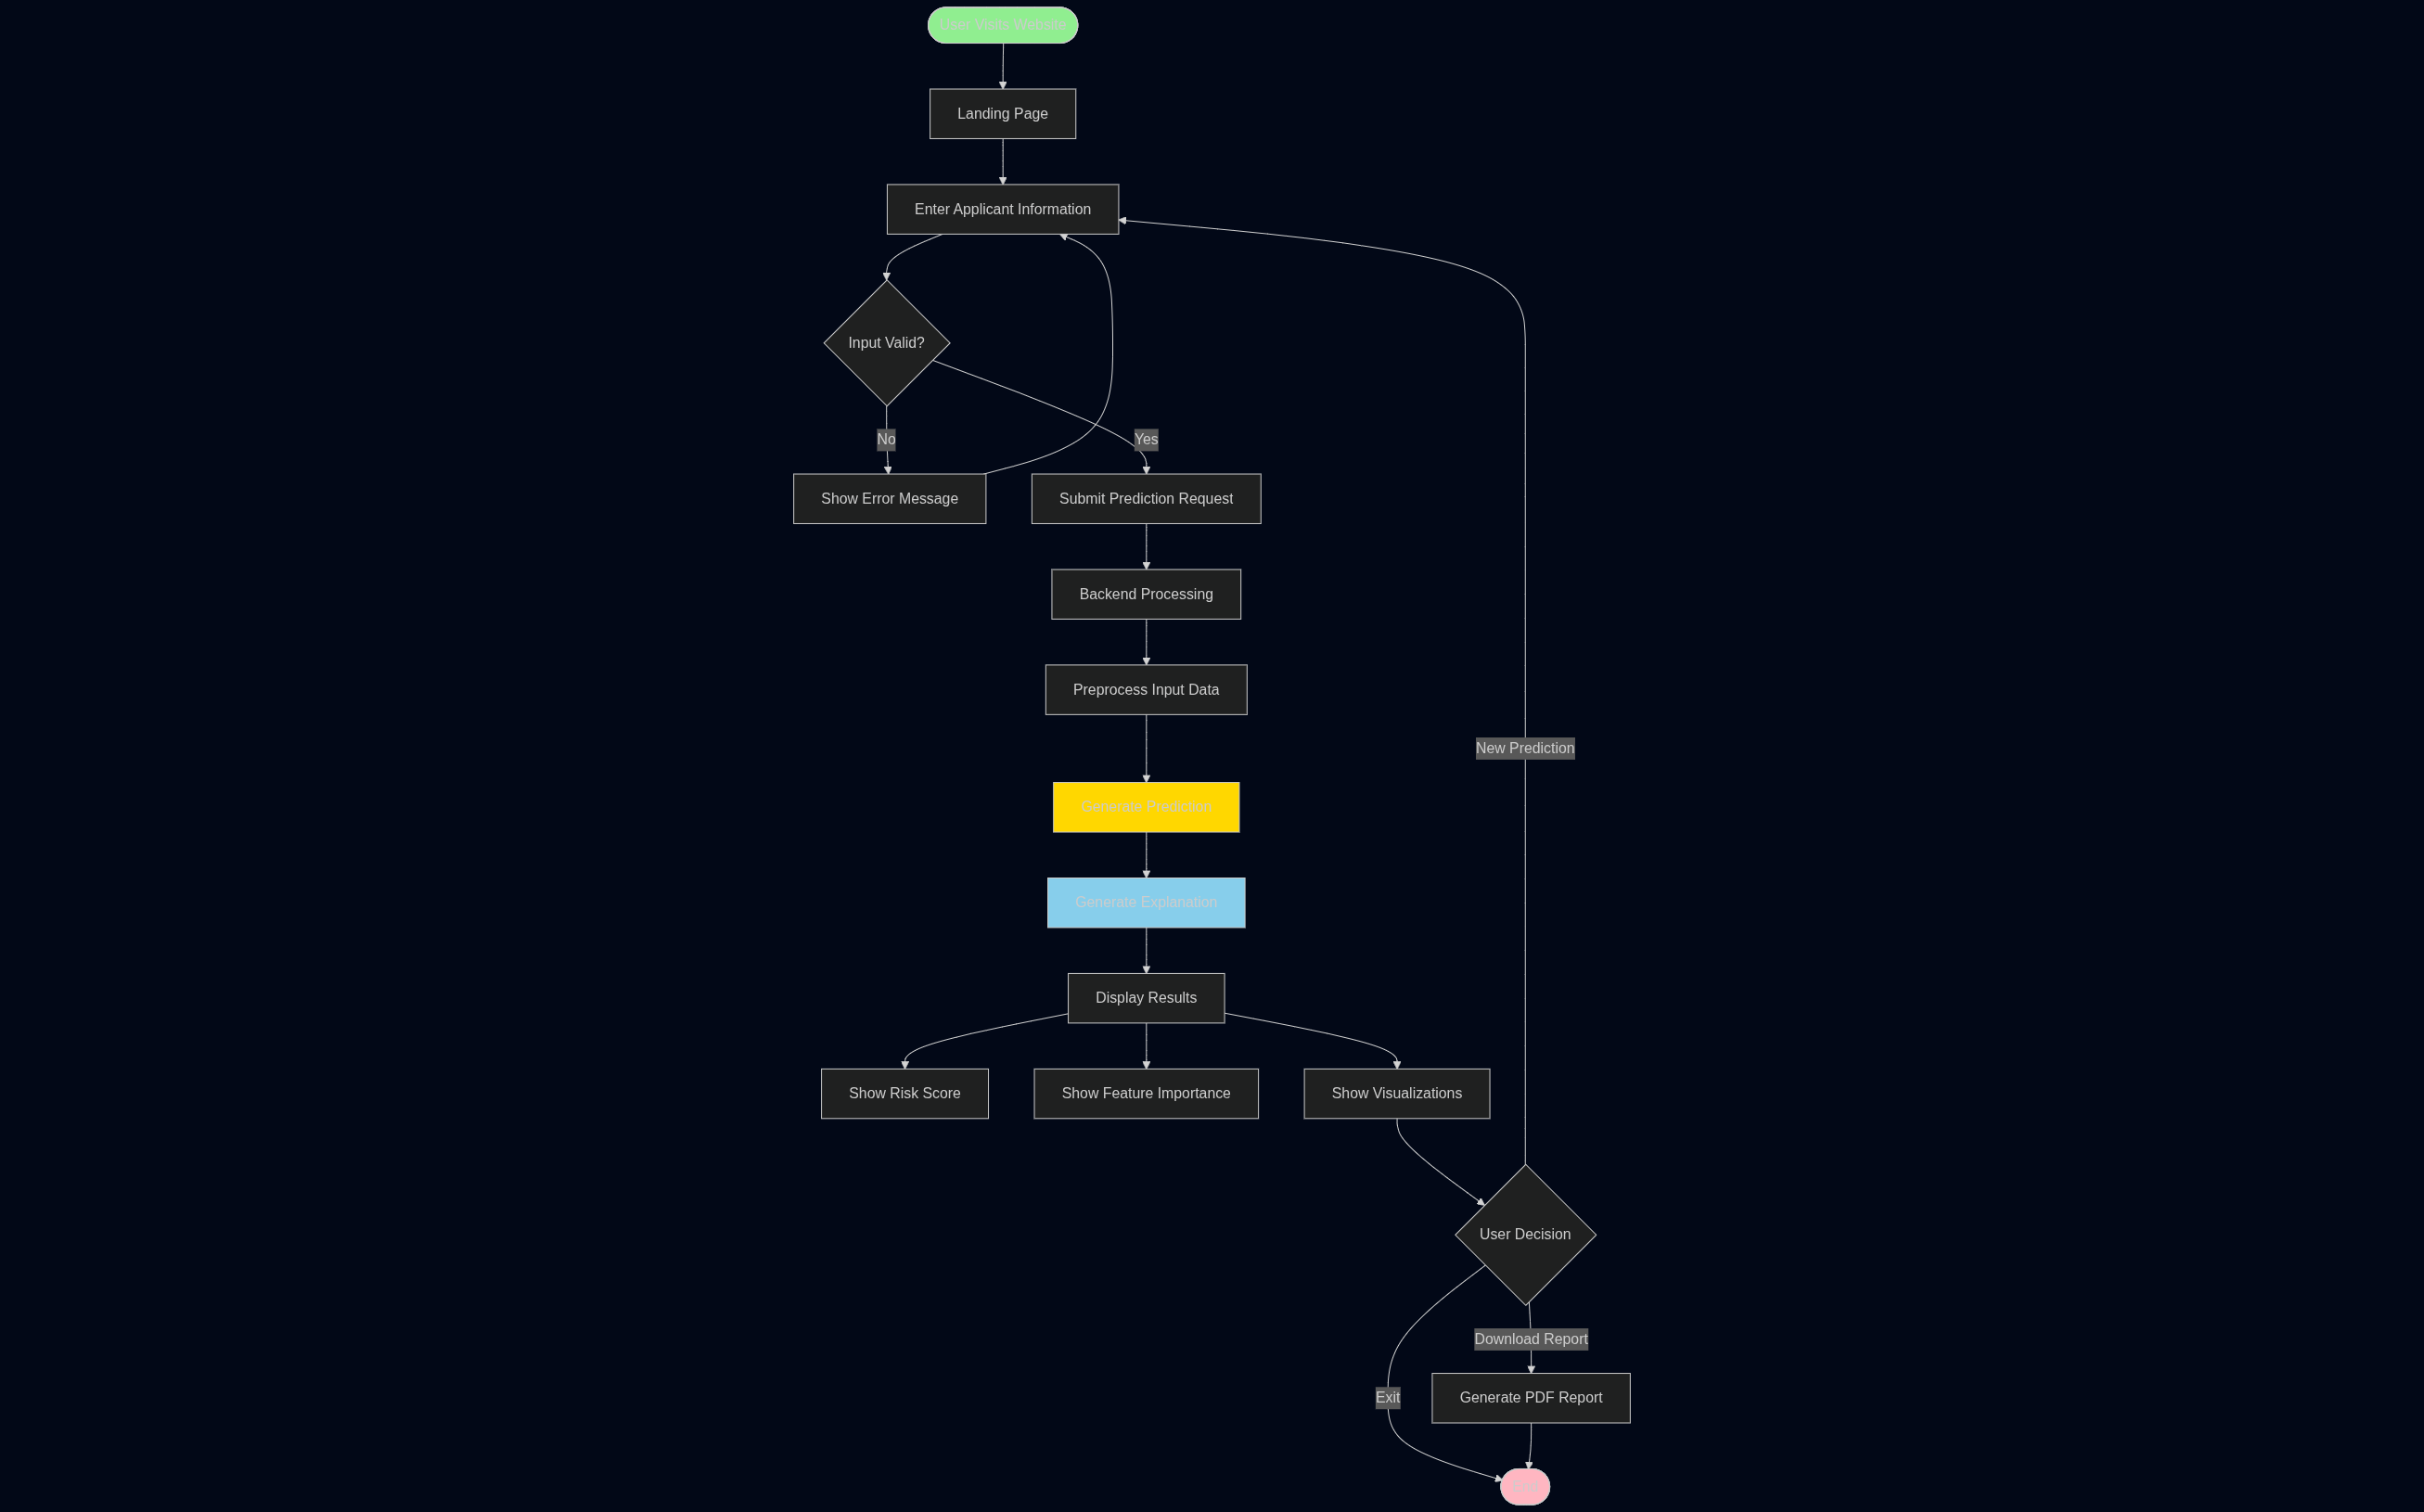
\includegraphics[width=0.75\textwidth,height=\textheight]{images/use-case-diagram.png}
\caption{Use Case Diagram}
\end{figure}

\begin{figure}
\centering
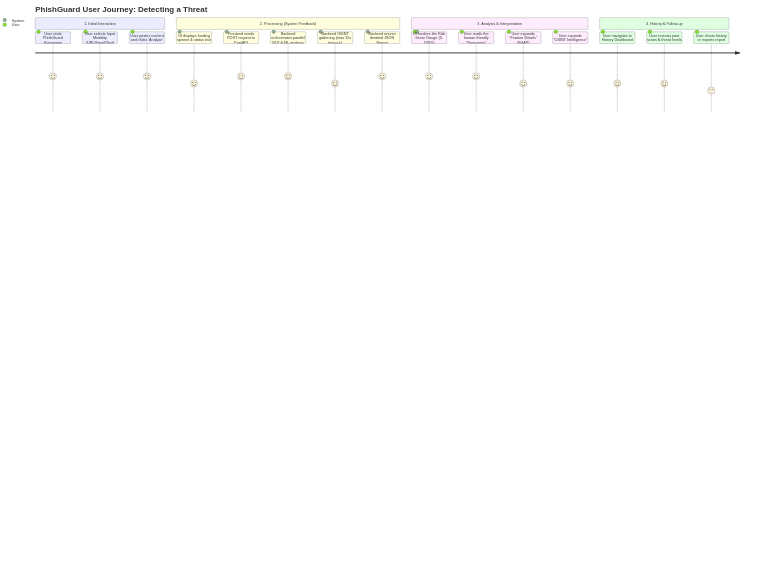
\includegraphics[width=0.75\textwidth,height=\textheight]{images/user-journey.png}
\caption{User Flow Diagram}
\end{figure}

\begin{figure}
\centering
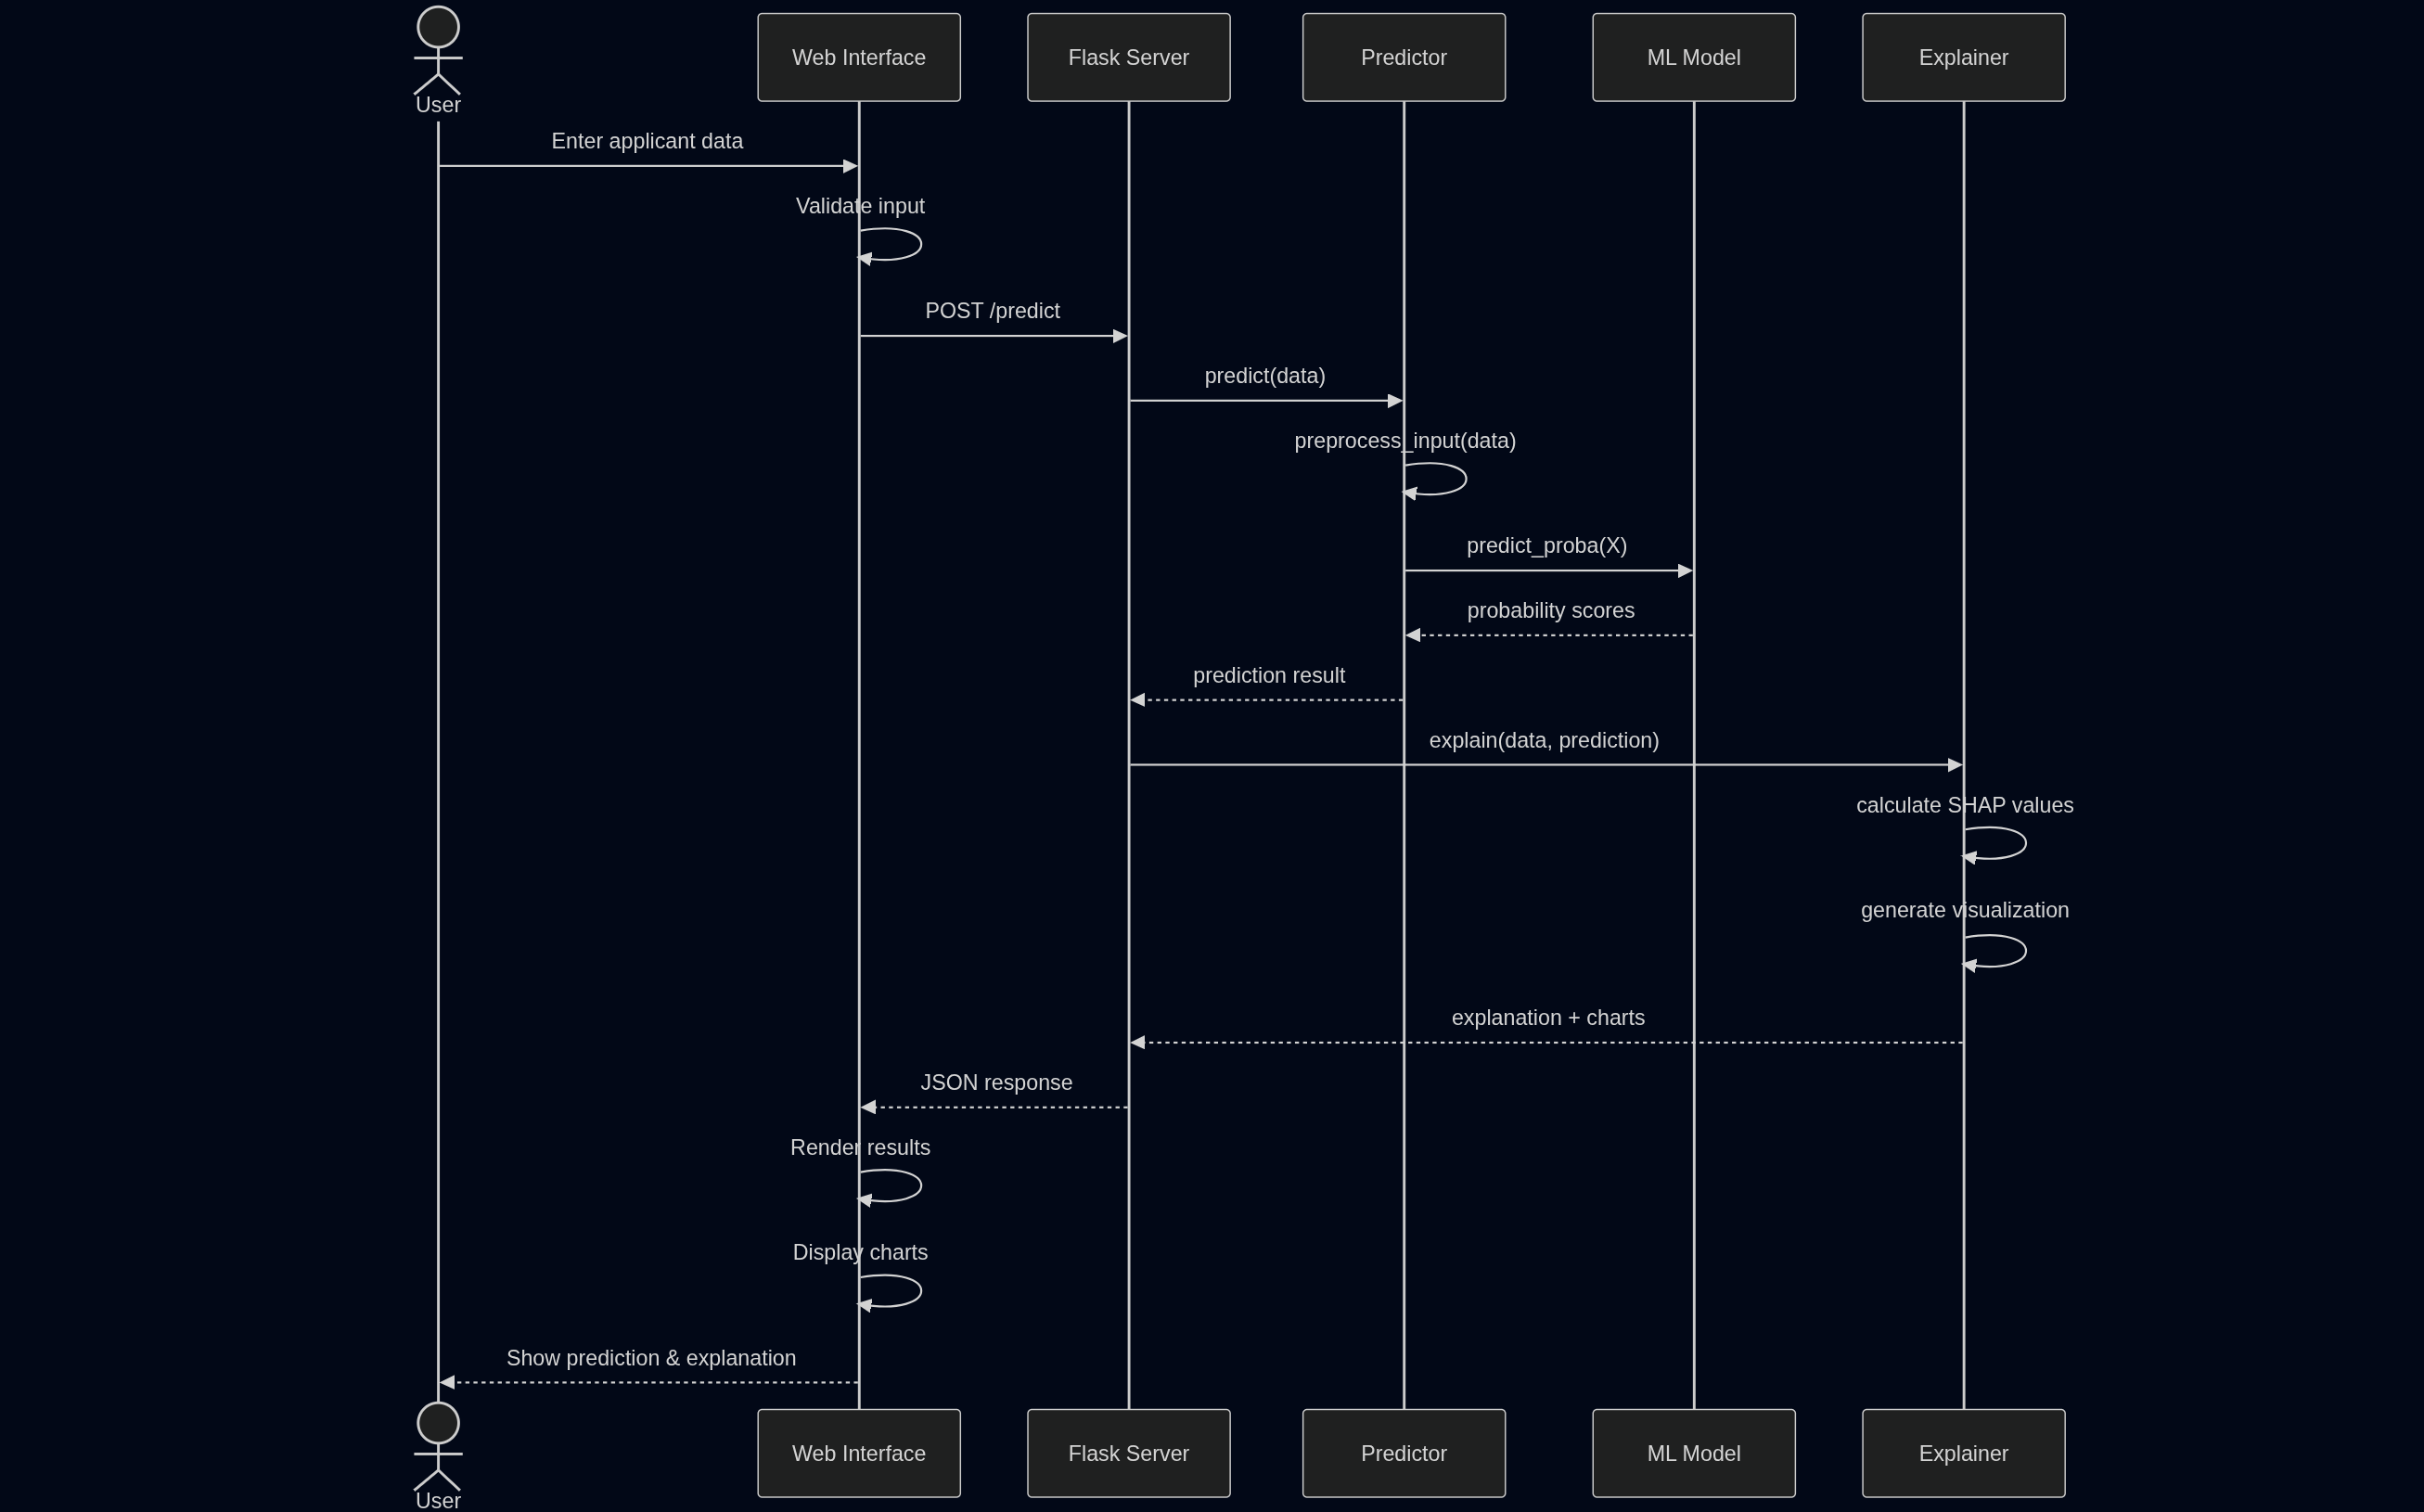
\includegraphics[width=0.75\textwidth,height=\textheight]{images/sequence-flow-diagram.png}
\caption{Sequence Diagram for Prediction Flow}
\end{figure}

\hypertarget{data-flow-component-state-and-class-diagrams}{%
\subsection{Data Flow, Component, State, and Class
Diagrams}\label{data-flow-component-state-and-class-diagrams}}

\begin{figure}
\centering
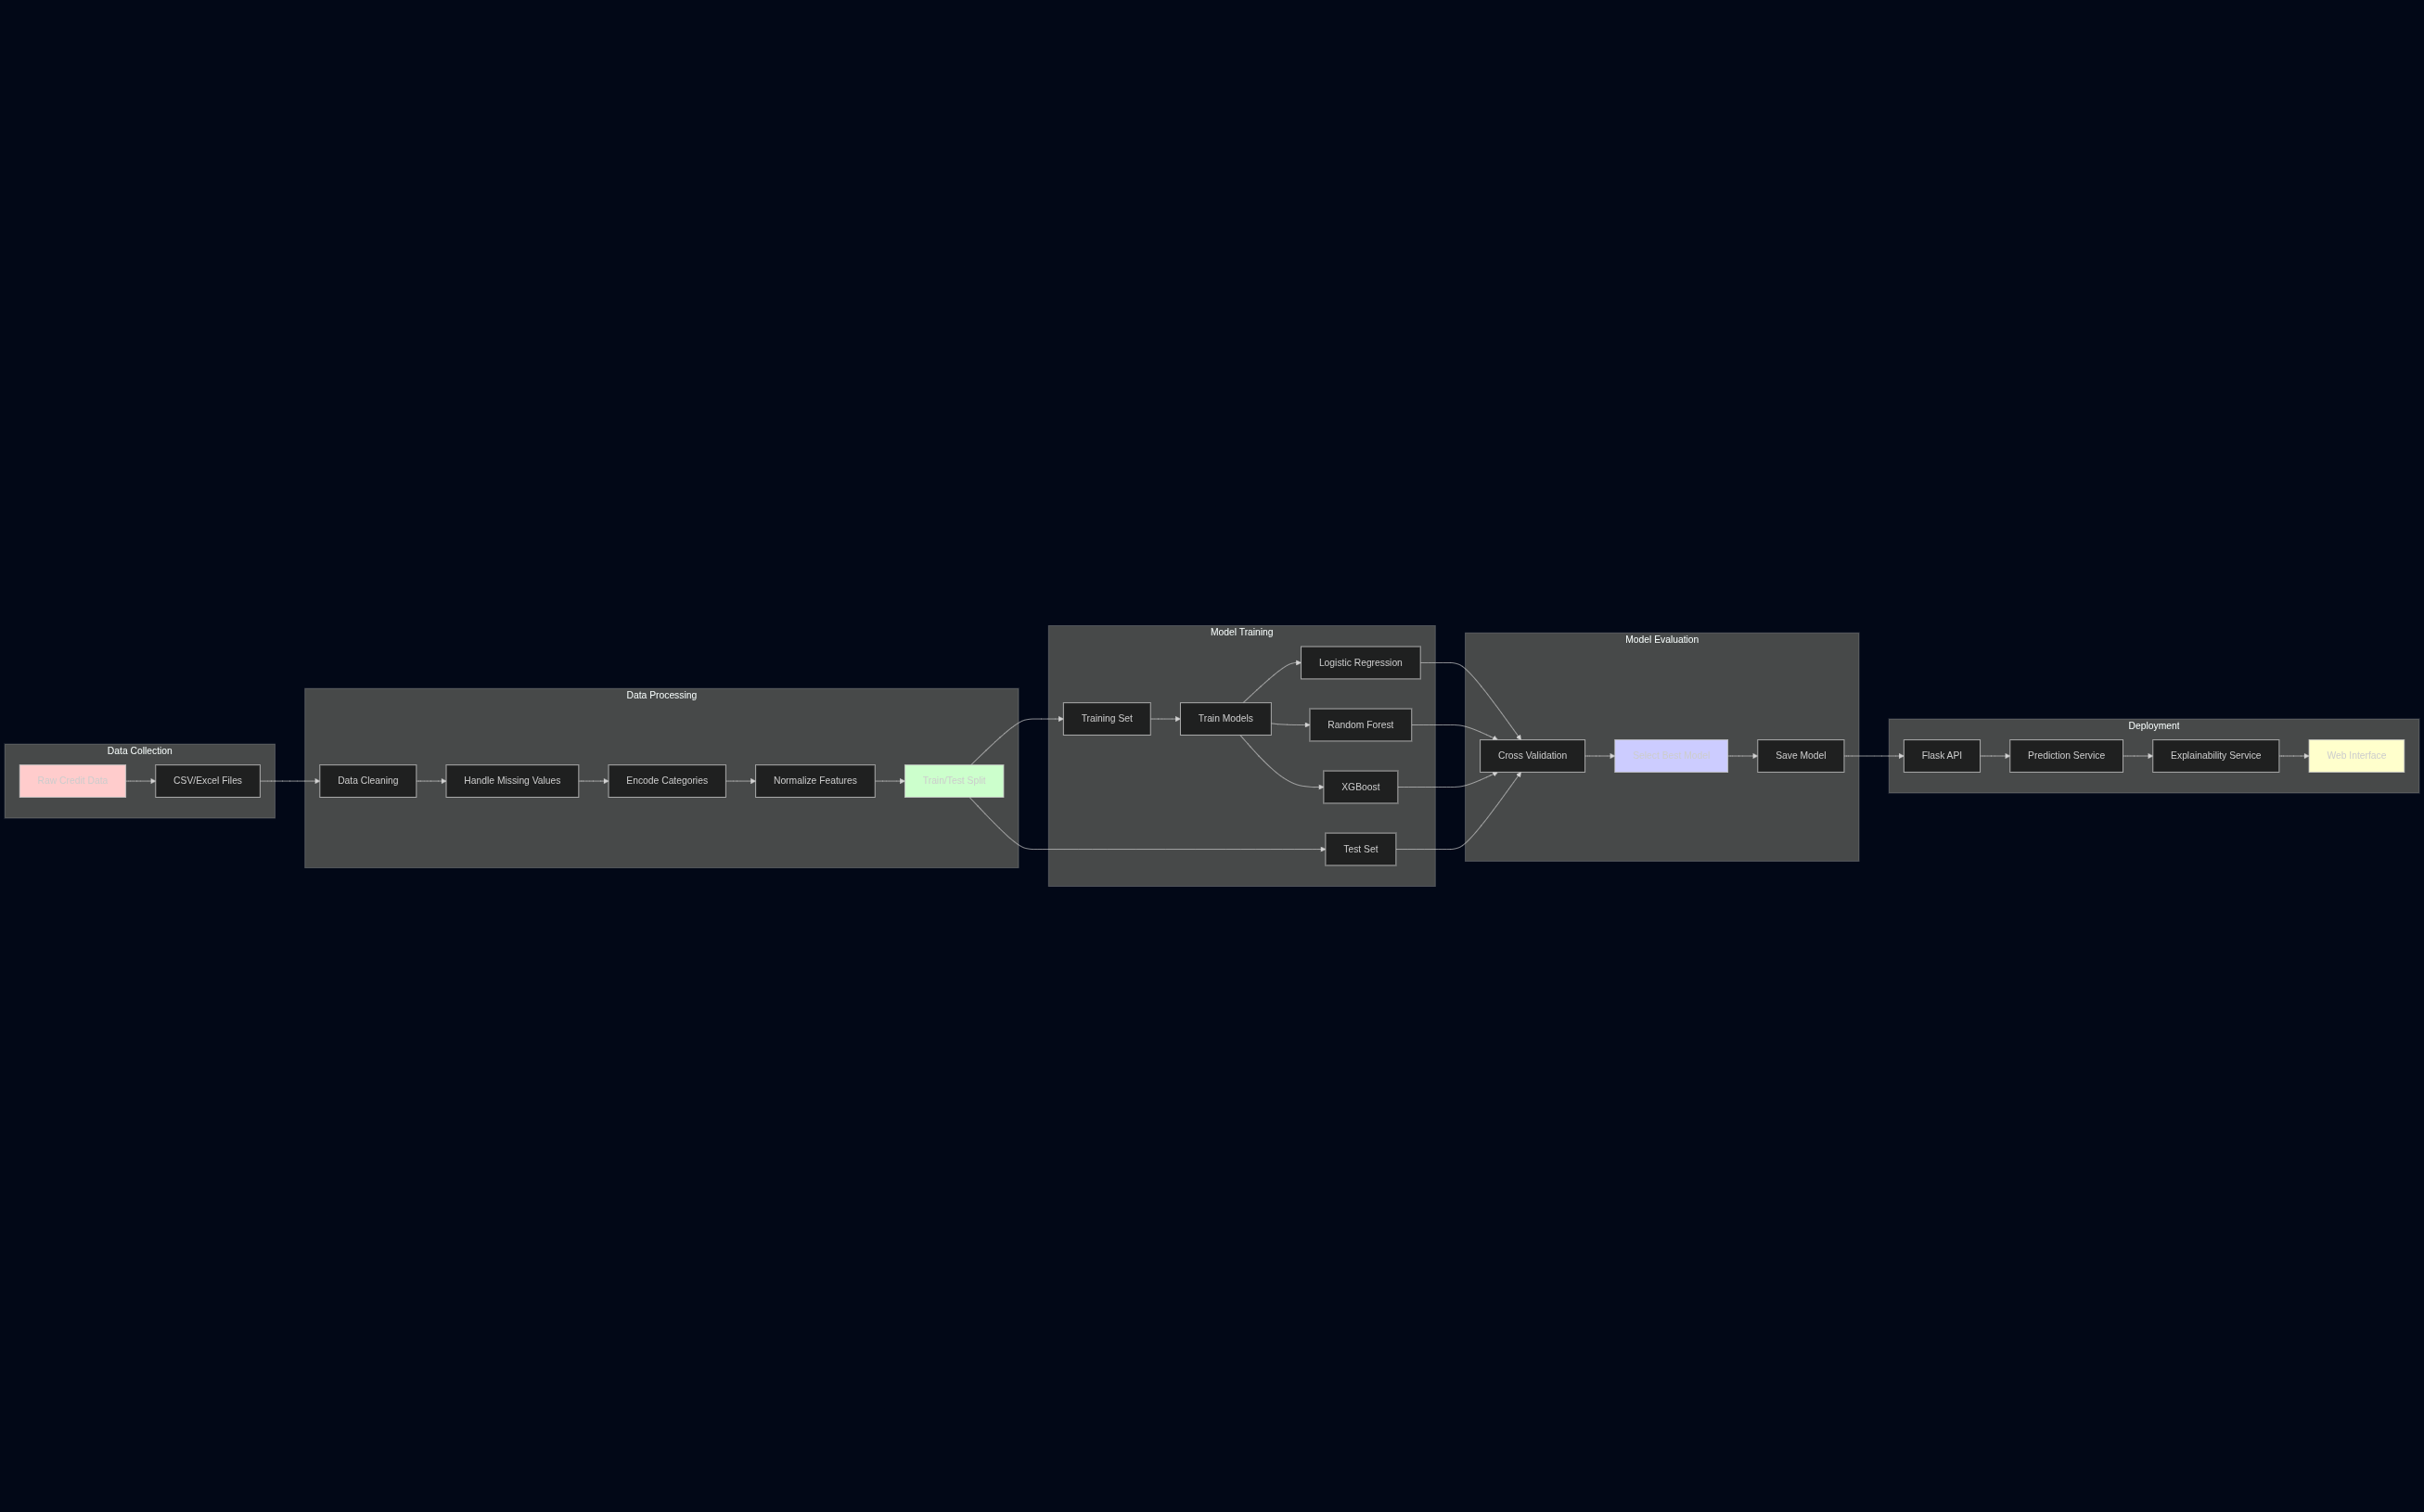
\includegraphics[width=0.75\textwidth,height=\textheight]{images/data-flow-diagram.png}
\caption{Data Flow Diagram}
\end{figure}

\begin{figure}
\centering
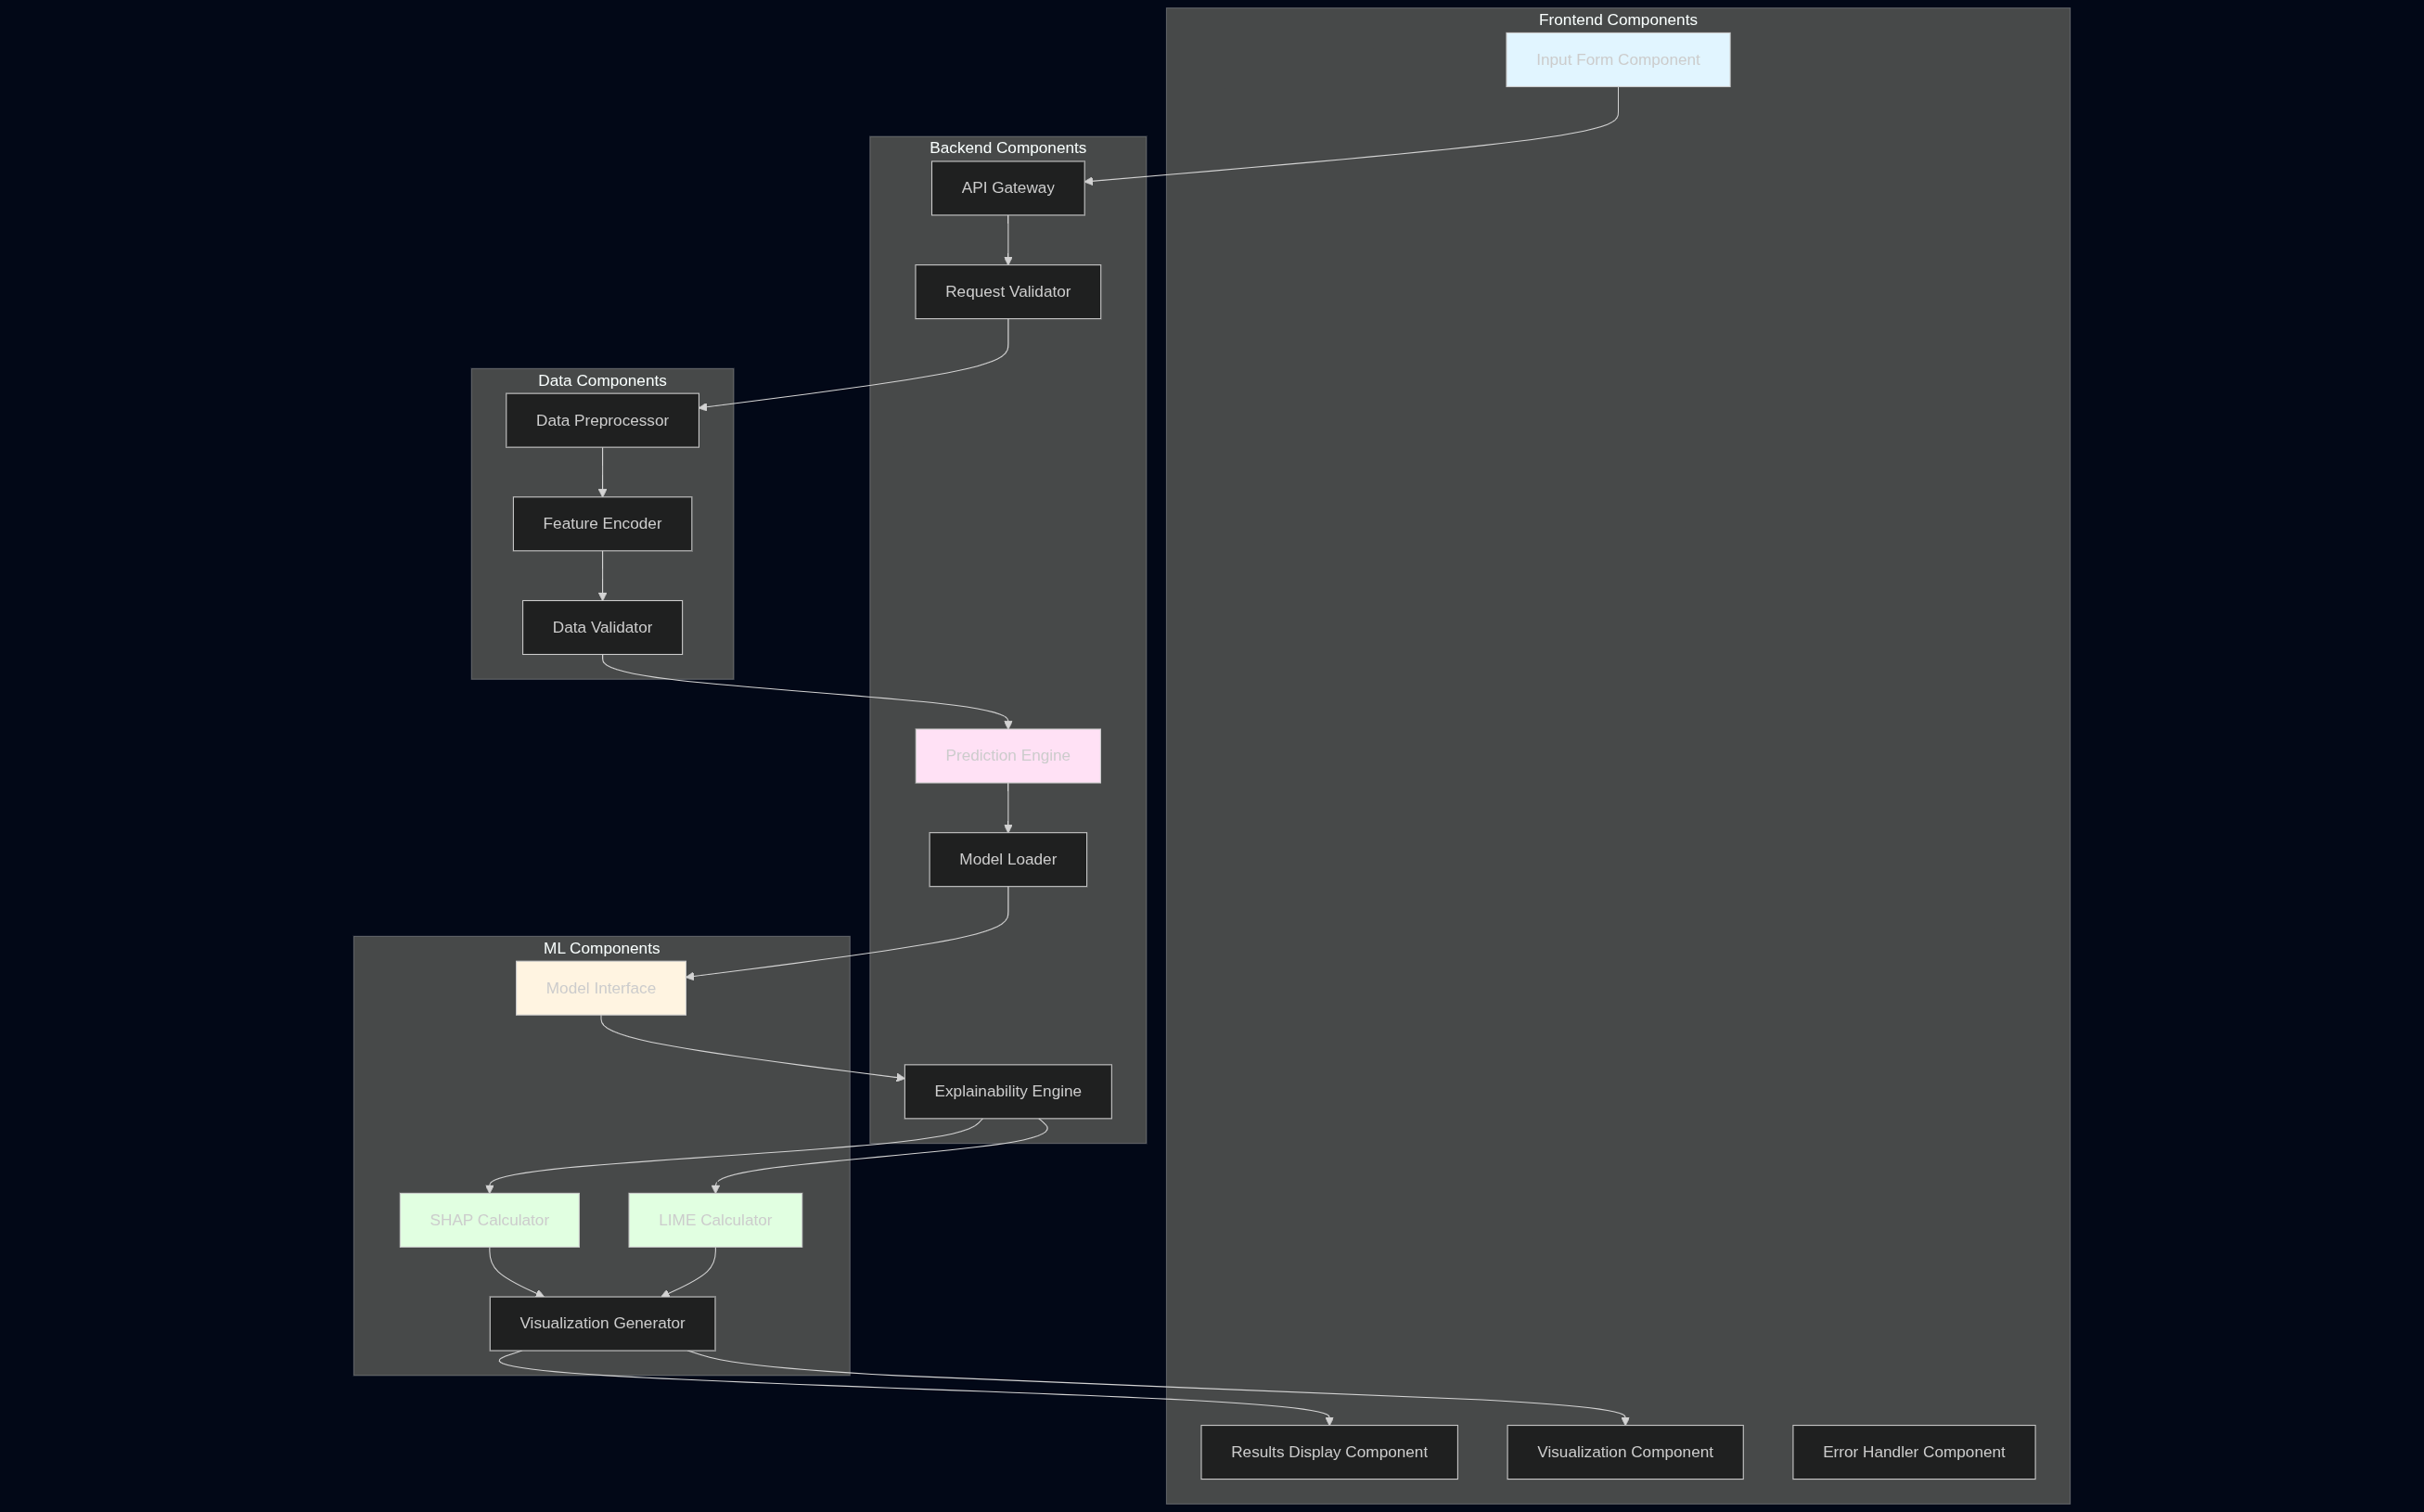
\includegraphics[width=0.75\textwidth,height=\textheight]{images/component-diagram.png}
\caption{Component Diagram}
\end{figure}

\begin{figure}
\centering
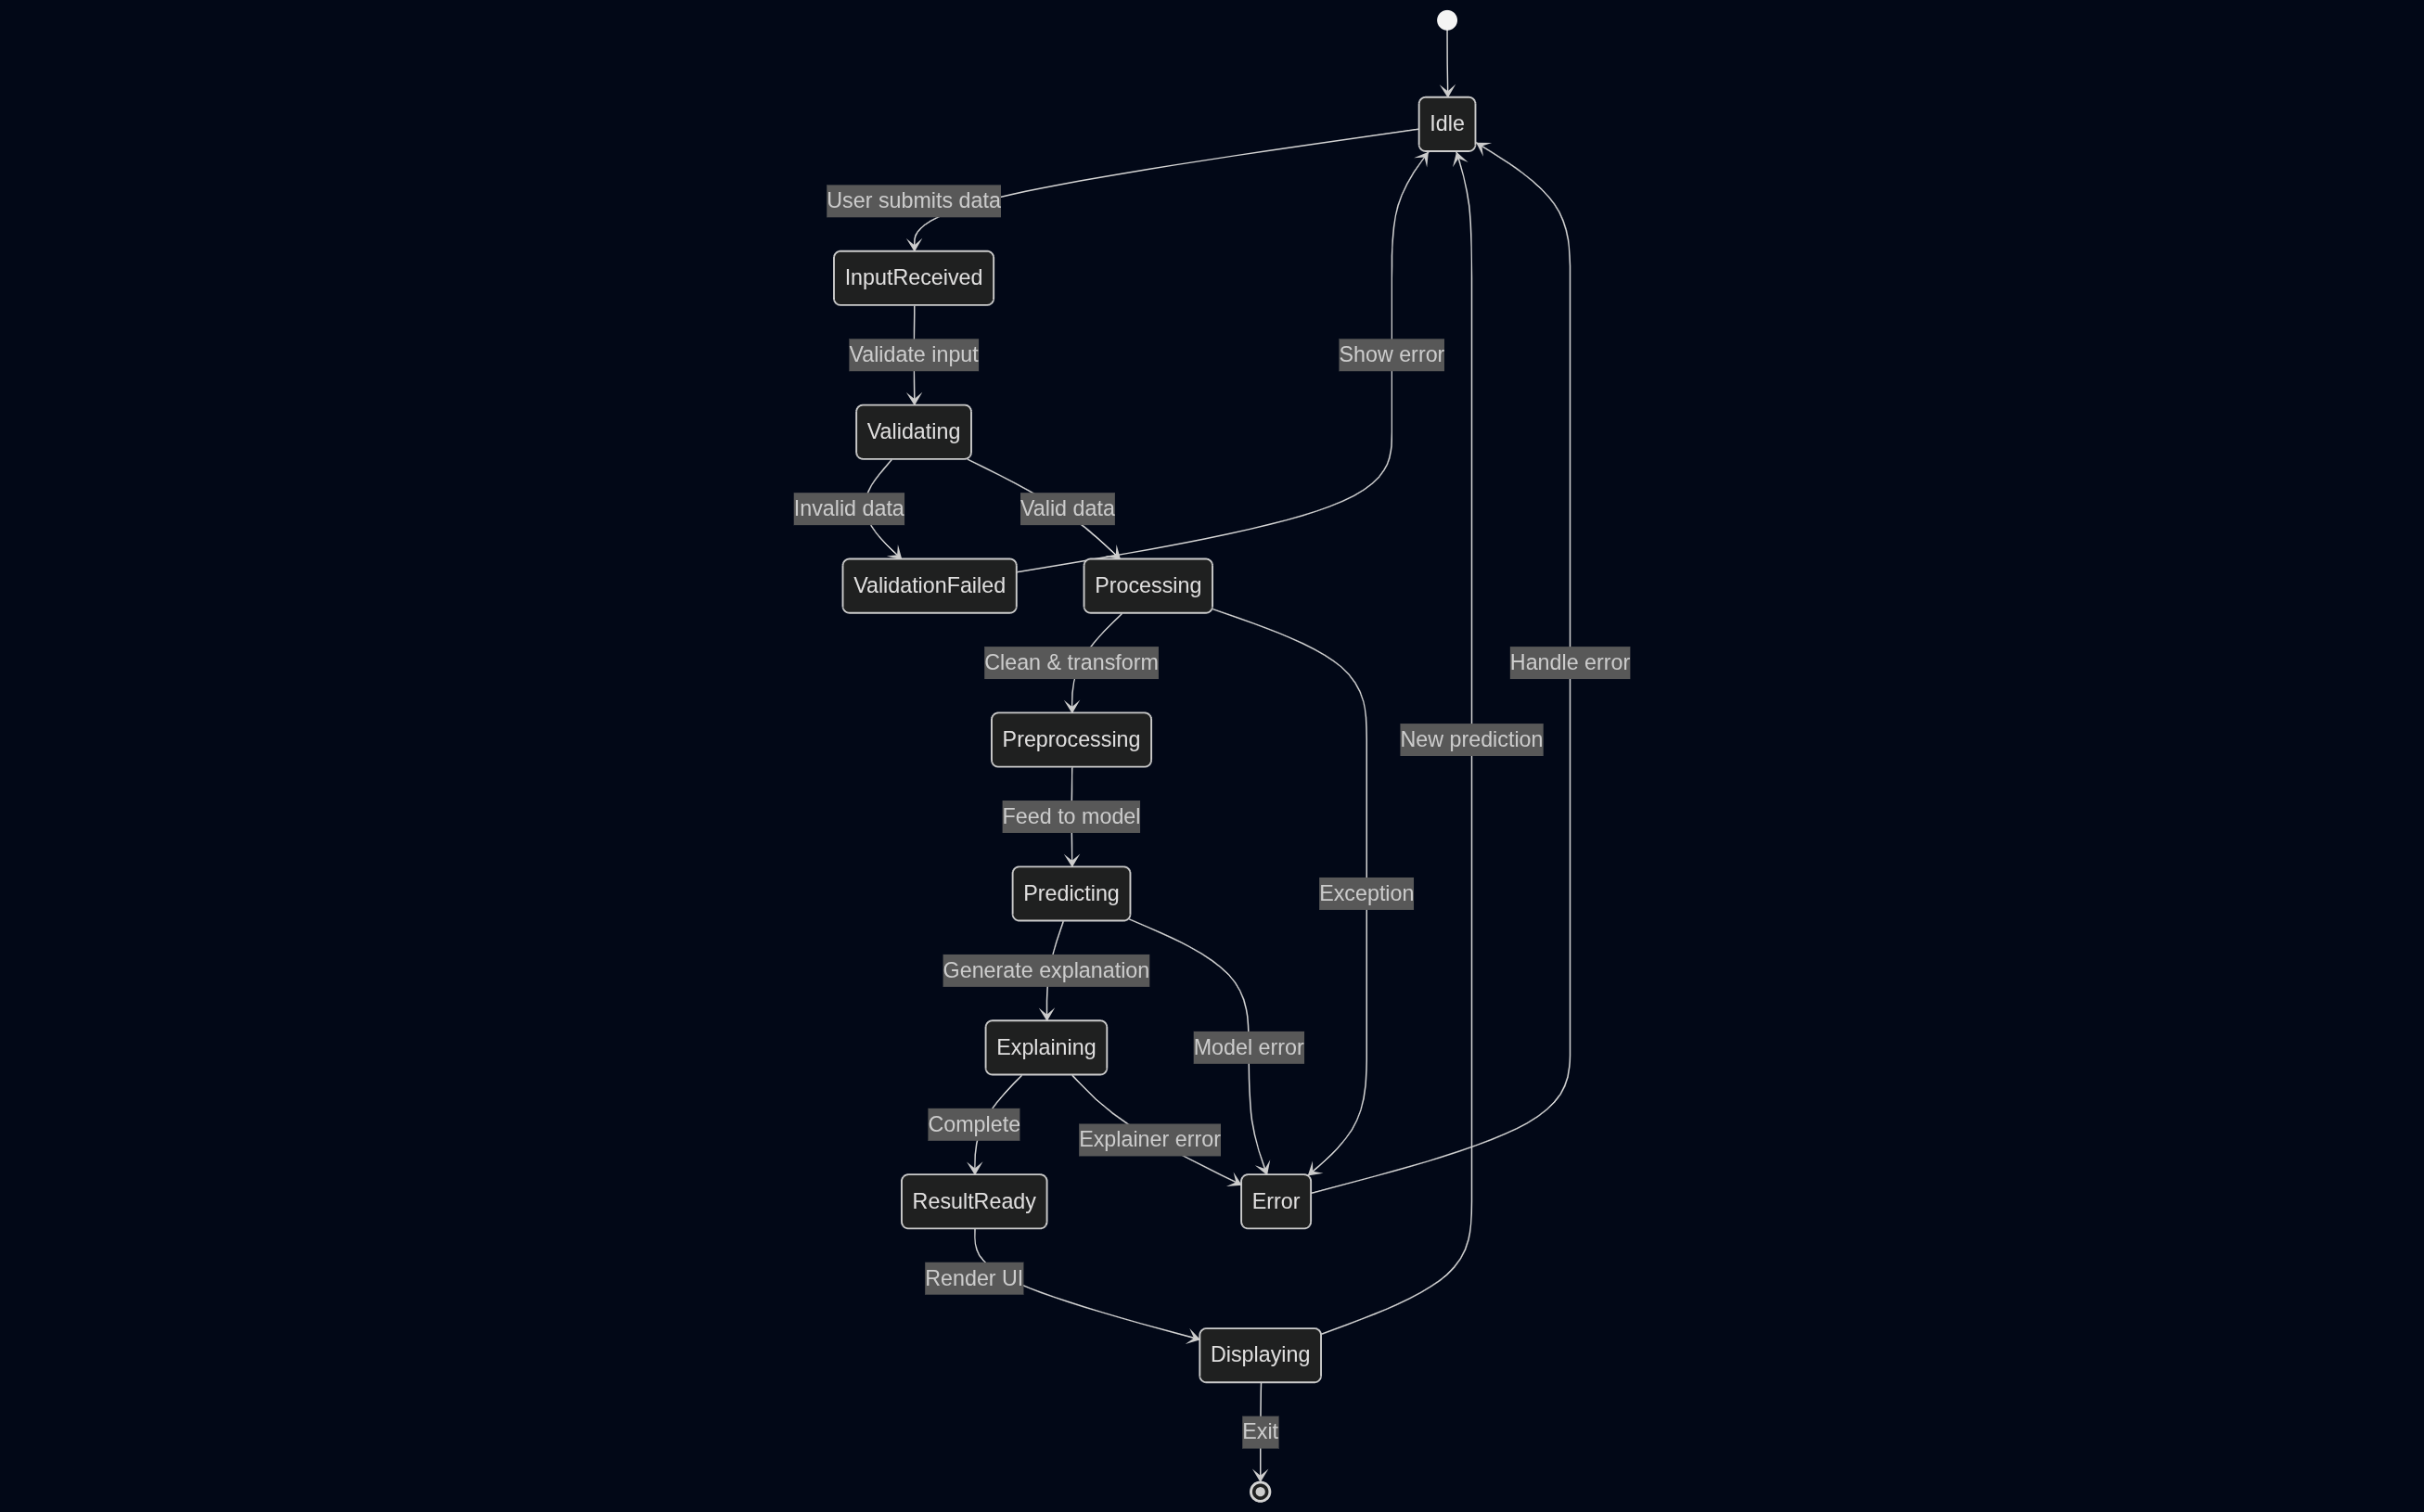
\includegraphics[width=0.75\textwidth,height=\textheight]{images/state-diagram.png}
\caption{State Diagram}
\end{figure}

\begin{figure}
\centering
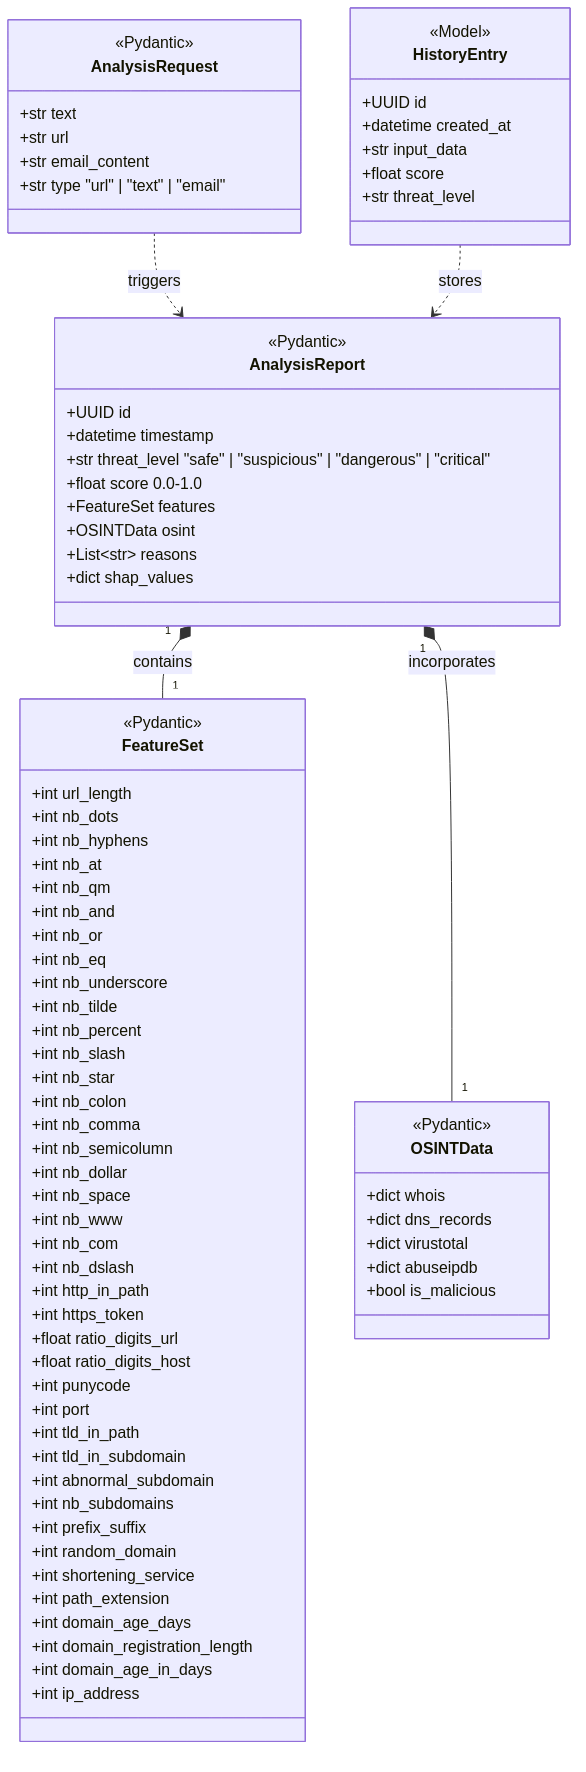
\includegraphics[width=0.75\textwidth,height=\textheight]{images/class-diagram.png}
\caption{Class Diagram}
\end{figure}

\hypertarget{system-and-machine-learning-architecture}{%
\subsection{System and Machine Learning
Architecture}\label{system-and-machine-learning-architecture}}

\begin{figure}
\centering
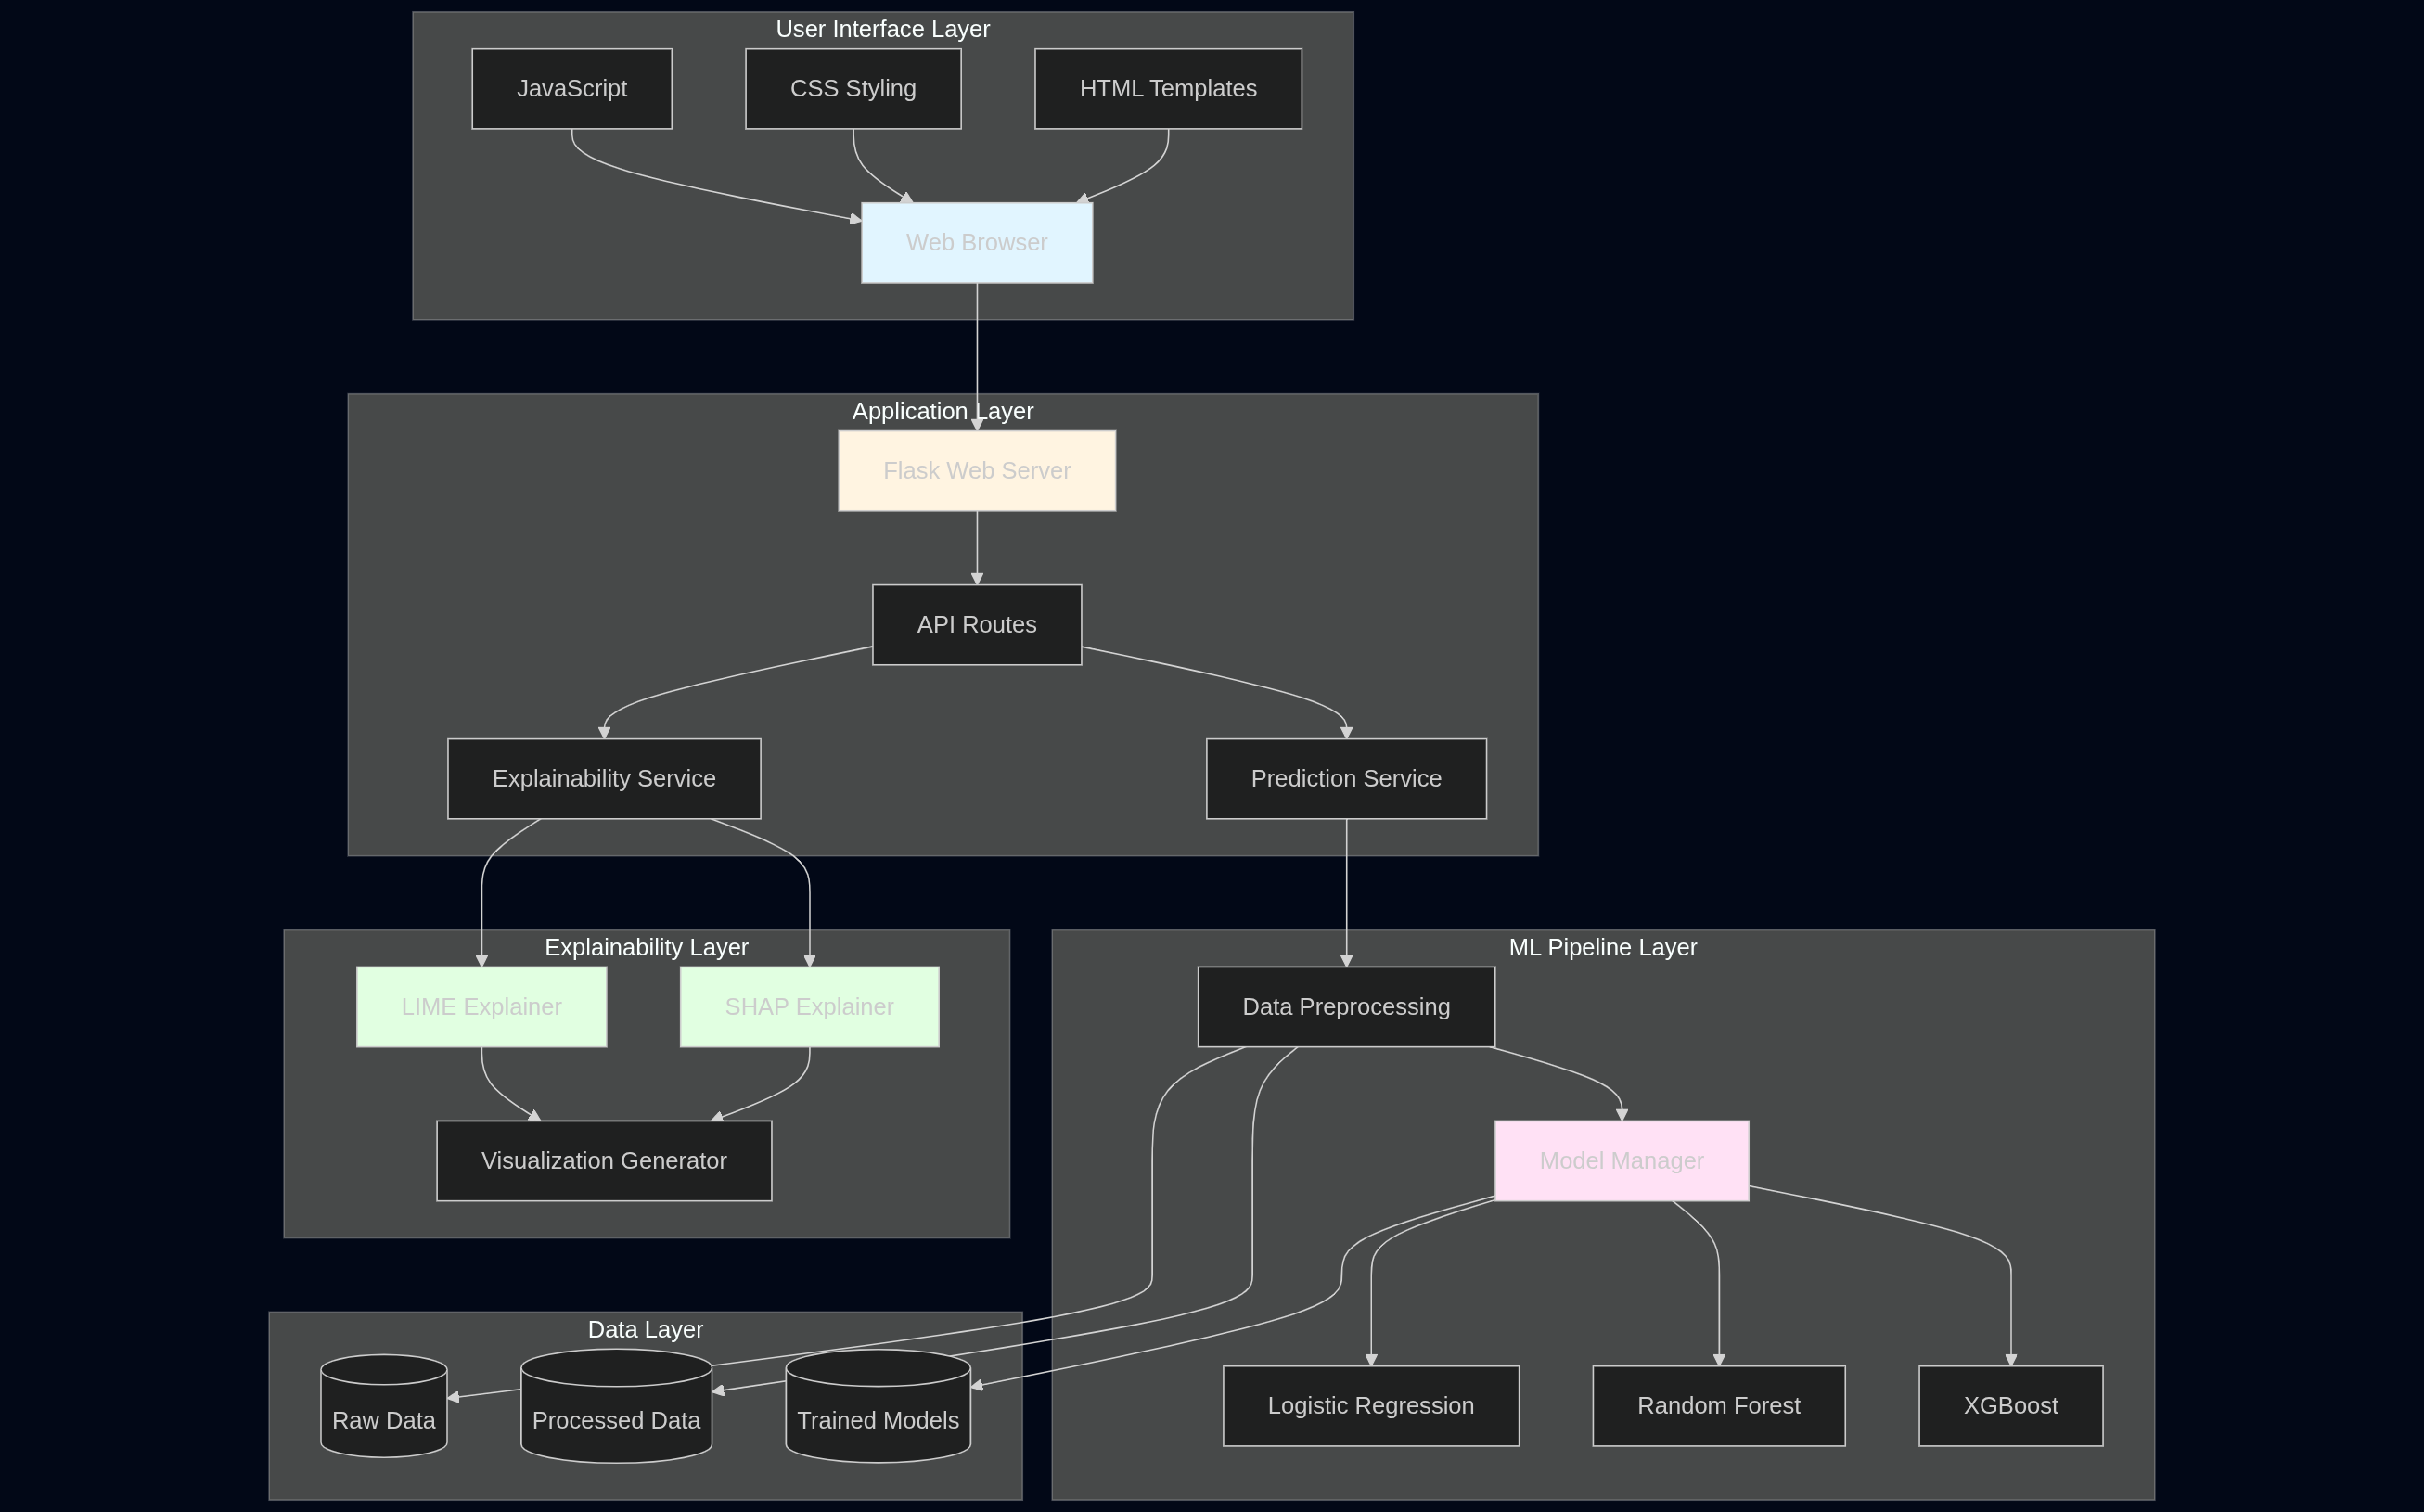
\includegraphics[width=0.75\textwidth,height=\textheight]{images/system-architecture-diagram.png}
\caption{System Architecture Diagram}
\end{figure}

\begin{figure}
\centering
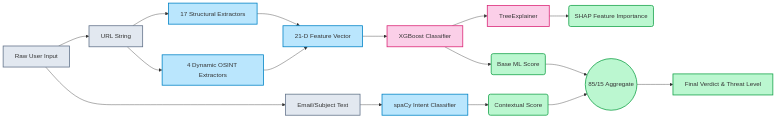
\includegraphics[width=0.75\textwidth,height=\textheight]{images/ml-pipeline.png}
\caption{Machine Learning Pipeline}
\end{figure}

\hypertarget{web-tool-screenshots}{%
\subsection{Web Tool Screenshots}\label{web-tool-screenshots}}

\begin{figure}[htbp]
\centering
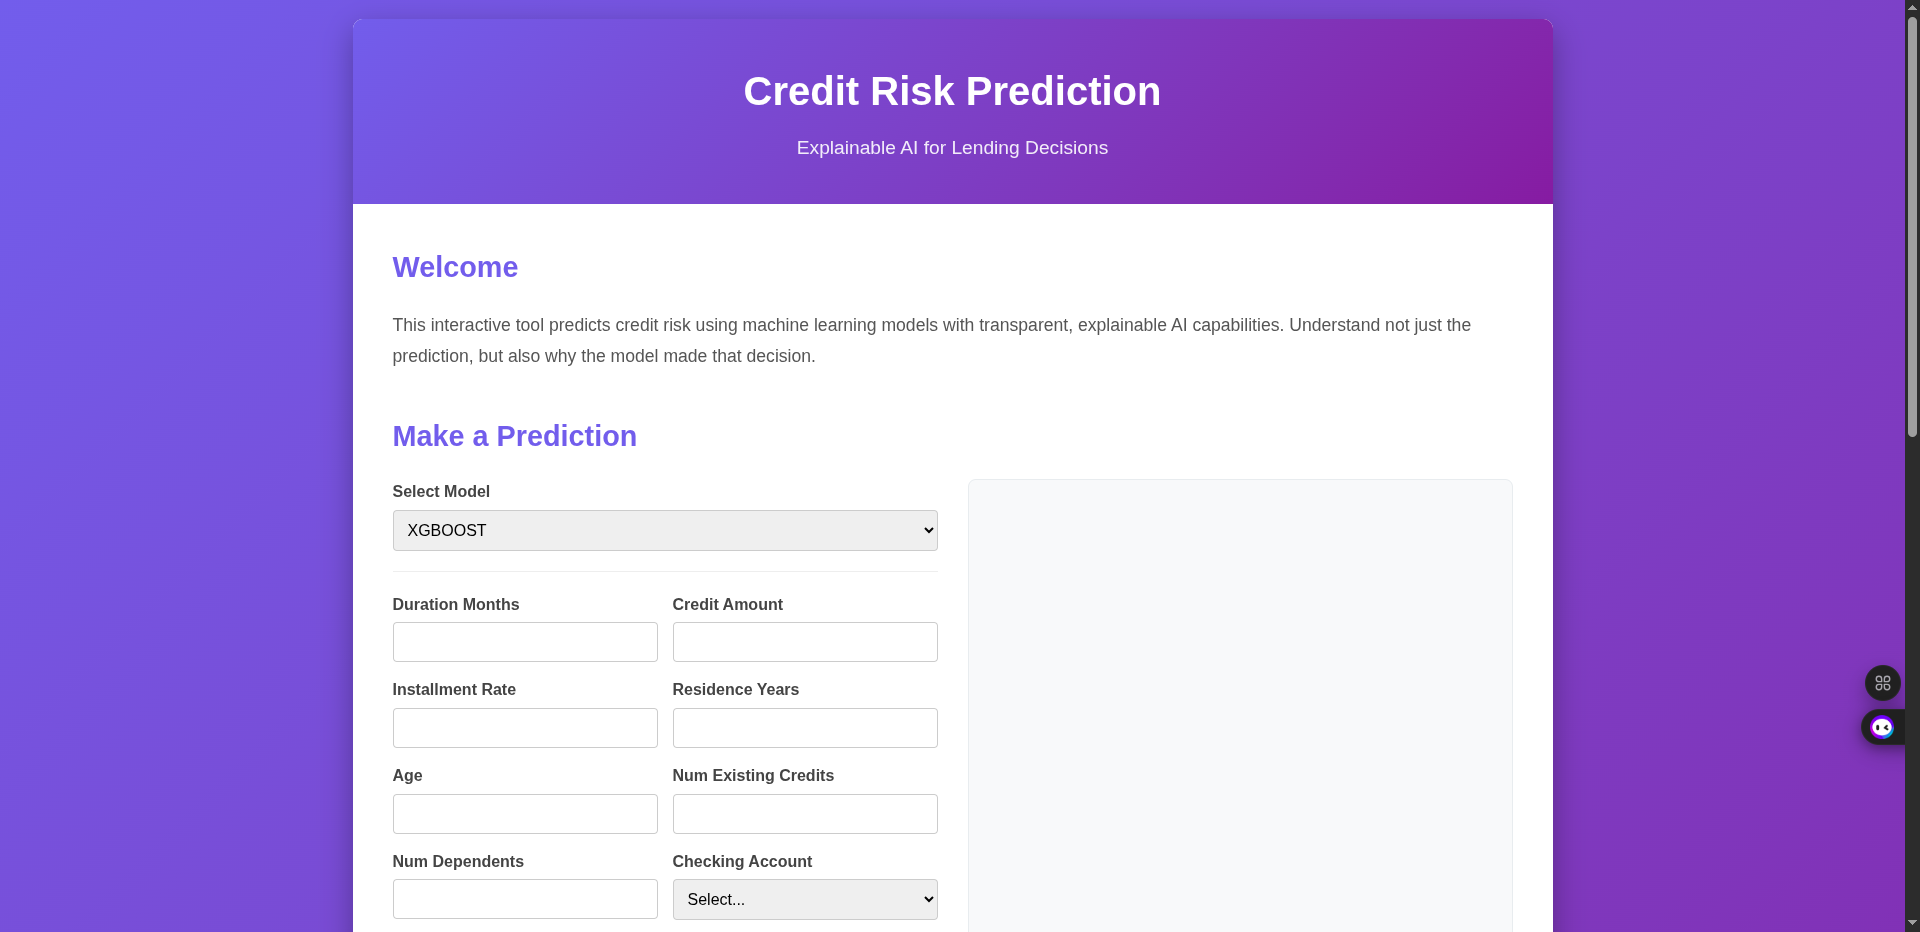
\includegraphics[width=0.75\textwidth,keepaspectratio]{images/web page 1.png}
\caption{Web Page Home Screenshot}
\end{figure}

\begin{figure}[htbp]
\centering
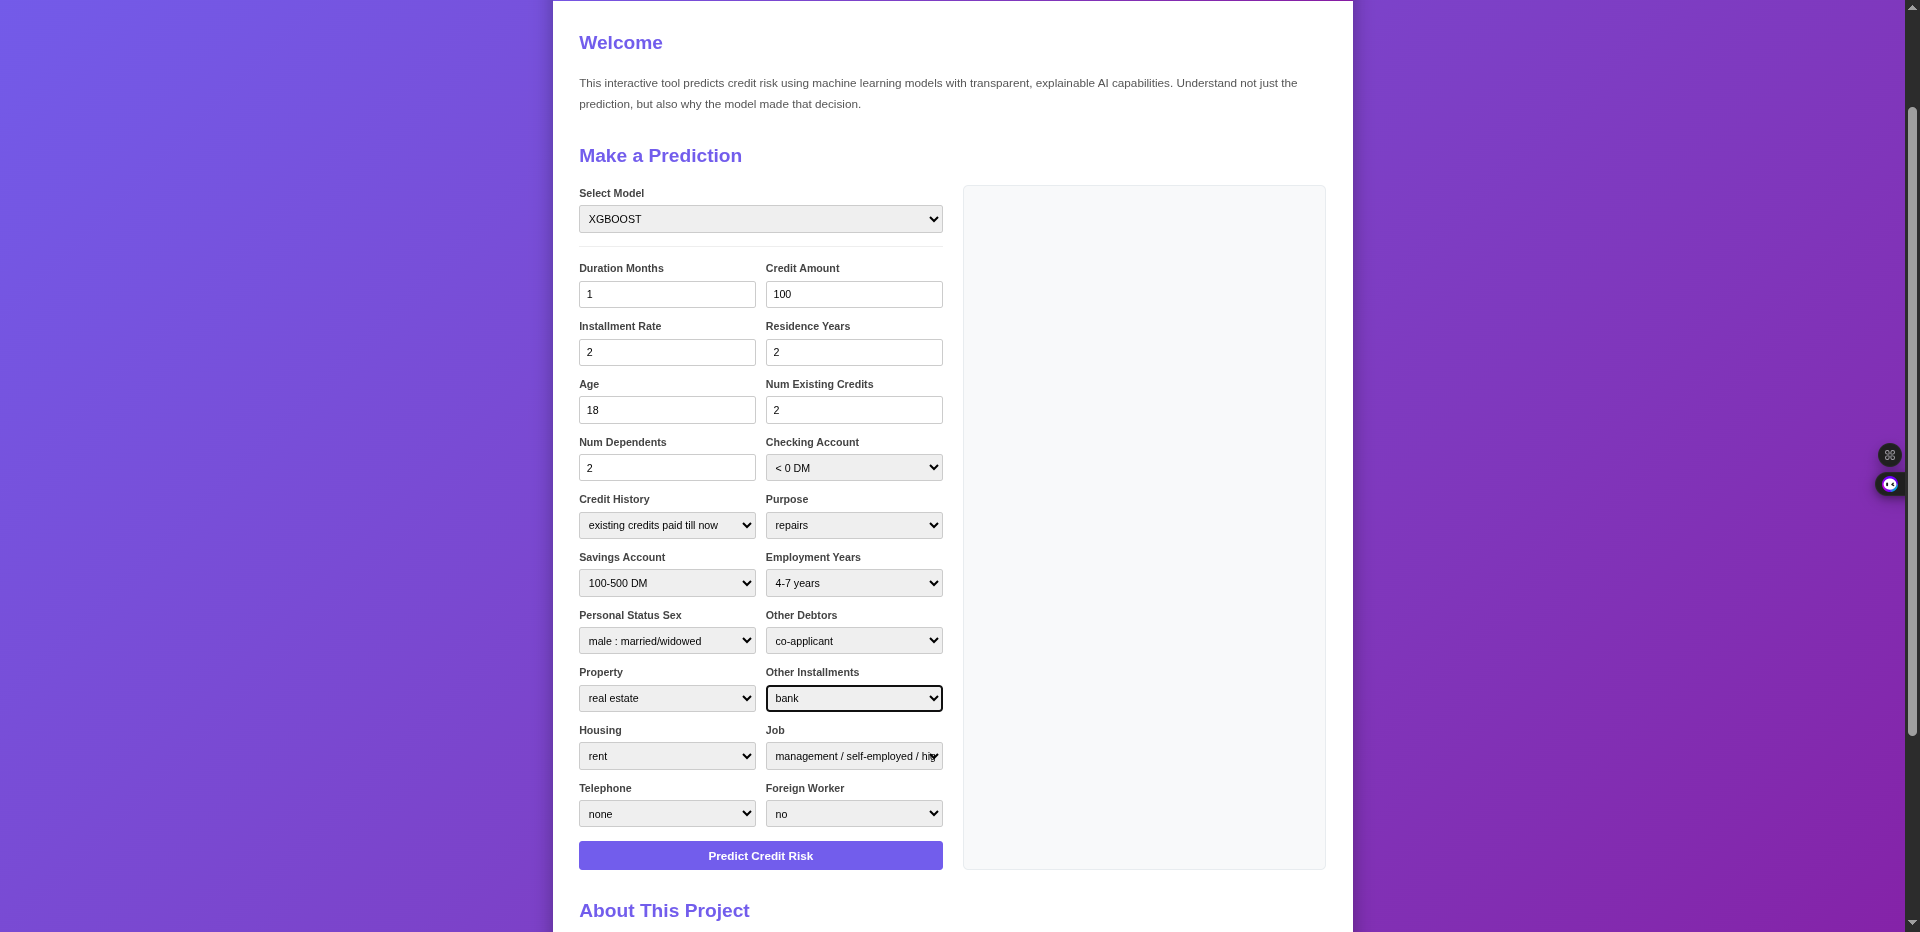
\includegraphics[width=0.75\textwidth,keepaspectratio]{images/filling the fields.png}
\caption{Form Filling Screenshot}
\end{figure}

\begin{figure}[htbp]
\centering
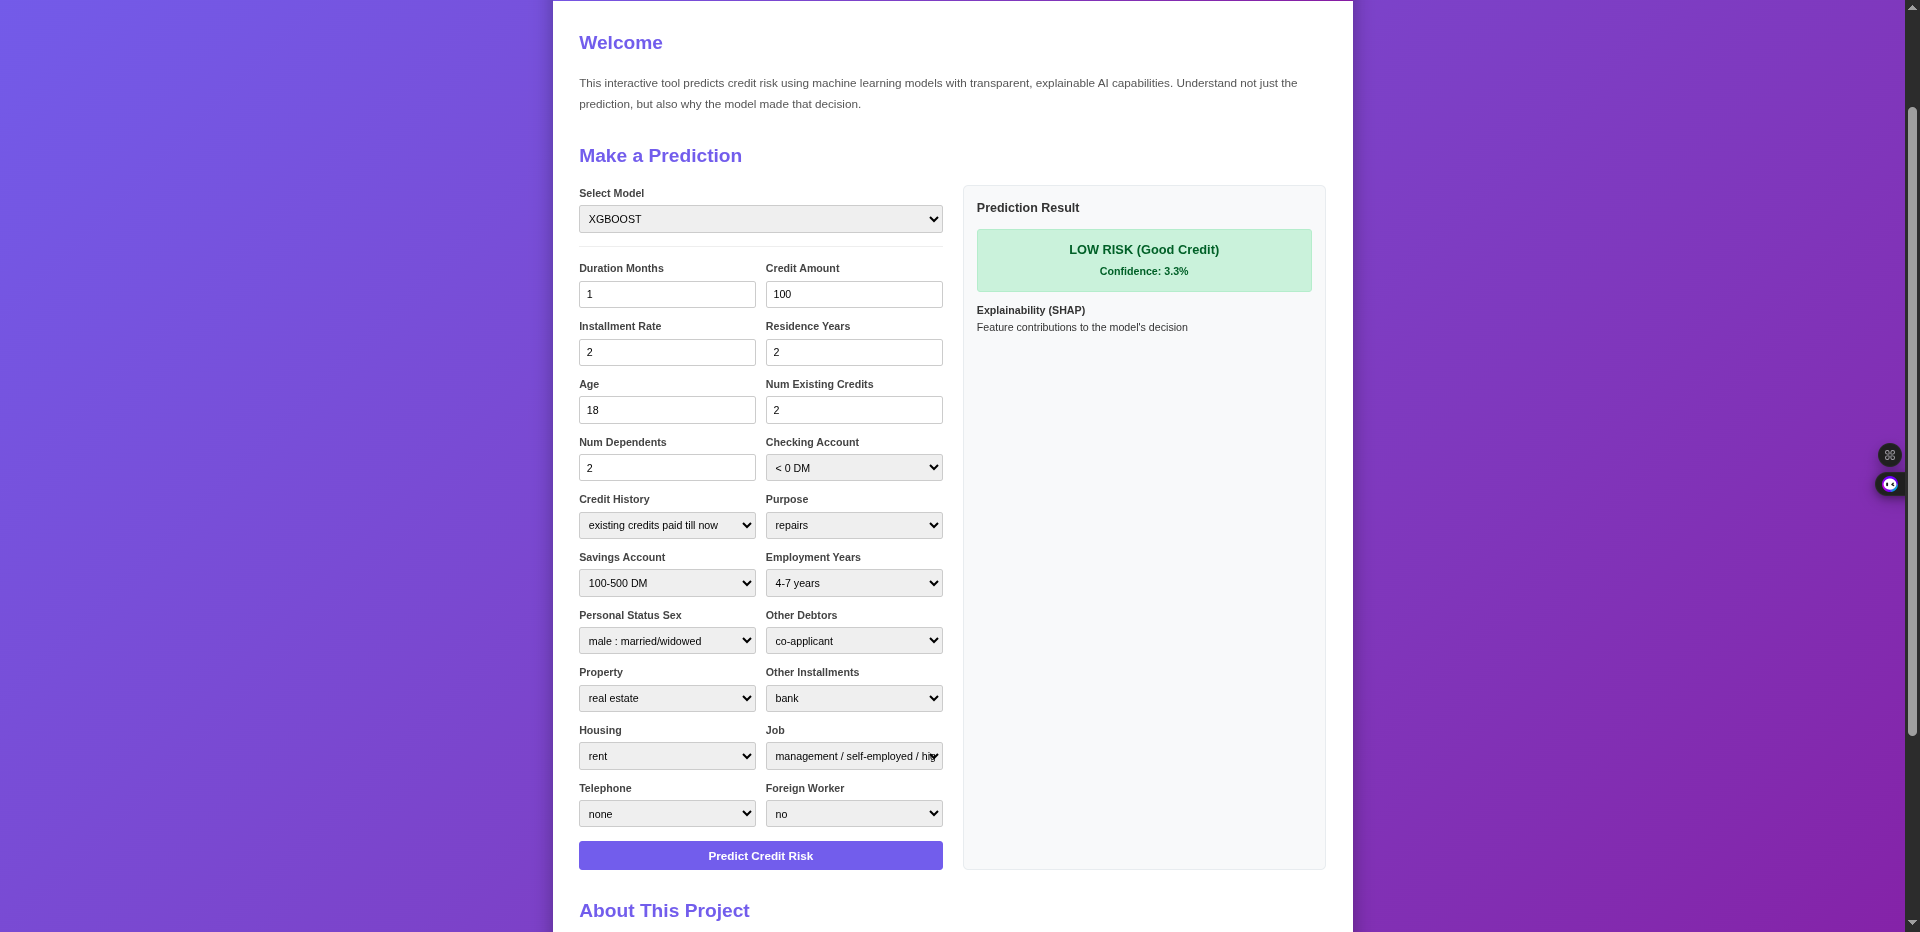
\includegraphics[width=0.75\textwidth,keepaspectratio]{images/results when you fill the fields.png}
\caption{Filled Form Result Screenshot}
\end{figure}

\begin{figure}[htbp]
\centering
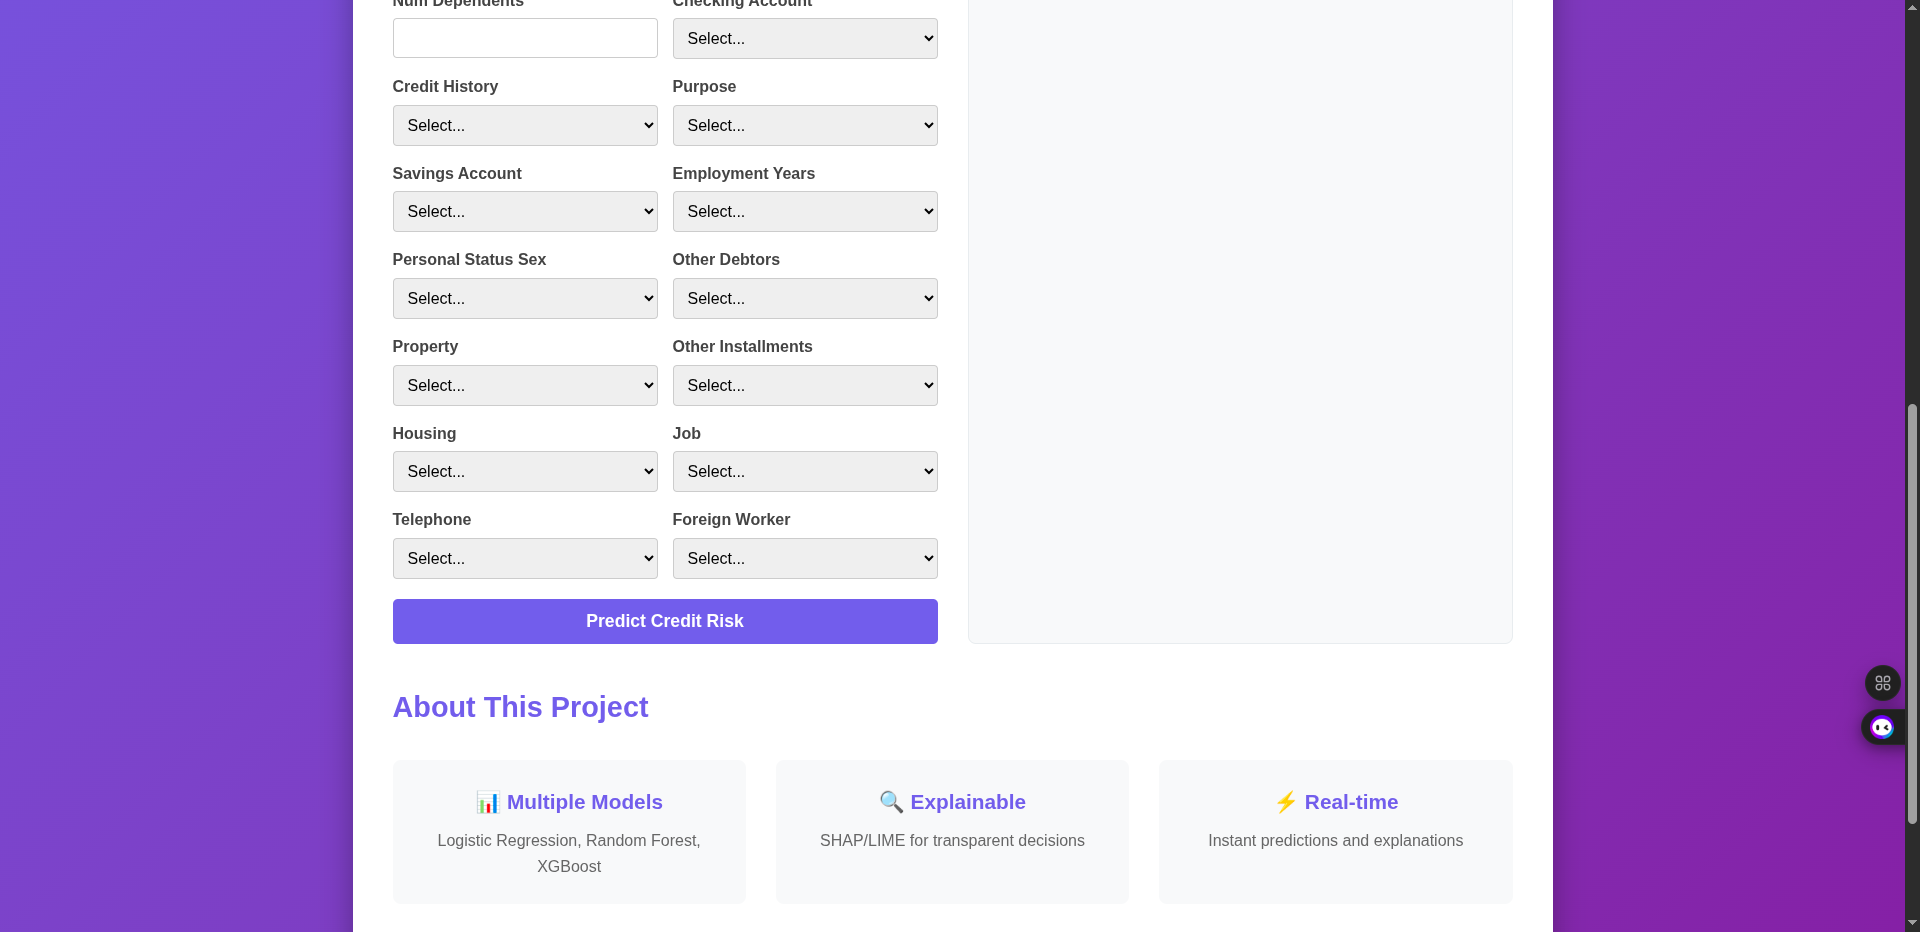
\includegraphics[width=0.75\textwidth,keepaspectratio]{images/web page 2.png}
\caption{Web Page Detail Screenshot}
\end{figure}

\hypertarget{testing-and-validation}{%
\section{Testing and Validation}\label{testing-and-validation}}

The implemented system was verified through automated unit and
integration-style checks that exercise the Flask application, the
prediction endpoint, and the surrounding preprocessing and inference
flow. The test suite is organized under the project \texttt{tests/}
directory and includes targeted coverage for the following layers:

\begin{itemize}
\tightlist
\item
  \texttt{tests/test\_app.py}: Flask route smoke tests and prediction
  payload validation.
\item
  \texttt{tests/test\_preprocessor.py}: preprocessing behavior and
  feature handling.
\item
  \texttt{tests/test\_training.py}: model training and persistence
  behavior.
\item
  \texttt{tests/test\_prediction.py}: inference path and output contract
  validation.
\item
  \texttt{tests/test\_explainability.py}: SHAP explanation generation.
\item
  \texttt{tests/test\_integration.py}: end-to-end workflow checks.
\end{itemize}

The screenshot below captures a successful execution of the web
application test suite:

\begin{figure}[htbp]
\centering
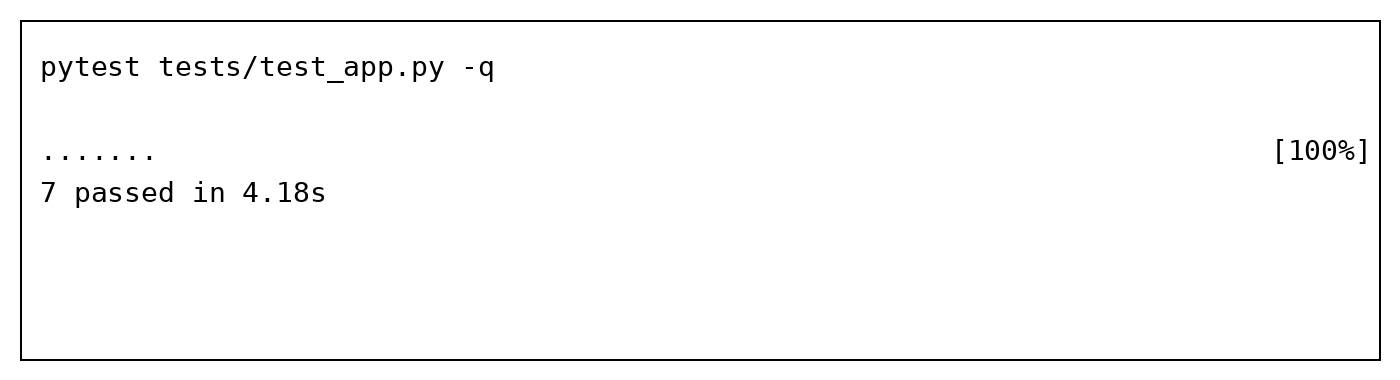
\includegraphics[width=0.75\textwidth,keepaspectratio]{images/test-results.png}
\caption{Unit Test Execution Result}
\end{figure}

\hypertarget{conclusion}{%
\chapter{Conclusion}\label{conclusion}}

The intersection of quantitative finance and artificial intelligence
presents one of the most intellectually demanding frontiers in modern
computer science. Historically, this domain has been paralyzed by a
fundamental dichotomy: algorithms possessing massive predictive capacity
operate as opaque mathematical black boxes, while transparent linear
models lack the geometric flexibility to map the true socio-economic
intricacies of human credit behavior. This thesis embarked upon a
rigorous methodological endeavor to structurally bridge this chasm,
architecting an end-to-end, production-grade machine learning platform
that explicitly unifies high-dimensional predictive classification with
cooperative game-theory interpretability.

\hypertarget{synthesis-of-contributions-and-concluding-remarks}{%
\subsection{Synthesis of Contributions and Concluding
Remarks}\label{synthesis-of-contributions-and-concluding-remarks}}

The foundational objective of this research was to empirically
demonstrate that modern ensemble mechanisms can be theoretically
validated, programmatically deployed, and ethically interpreted within a
singular, decoupled software ecosystem.

\begin{enumerate}
\def\labelenumi{\arabic{enumi}.}
\tightlist
\item
  \textbf{Theoretical and Empirical Validation}: By mathematically
  dissecting baseline structures (Logistic Regression) against
  high-variance ensembles (Random Forest, XGBoost), the research
  established a definitive computational hierarchy. Through the rigorous
  application of Synthetic Minority Over-sampling Techniques (SMOTE) and
  \(k\)-fold stratified hyperparameter grid searching, the final
  serialized Random Forest architecture achieved a highly robust,
  generalized \textbf{\(0.820\) AUC-ROC} score on the Statlog credit
  topology. It structurally trapped \(\approx 80\%\) of actual
  defaulting profiles, maximizing statistical Recall while fundamentally
  protecting institutional portfolio capital against catastrophic Type
  II errors.
\item
  \textbf{Systemic Architectural Decoupling}: The thesis transcended
  abstract Jupyter Notebook experimentation by engineering a rigid,
  stateless RESTful Application Programming Interface (API) utilizing
  the Flask micro-framework. By aggressively caching serialized binary
  \texttt{.pkl} memory artifacts into the Python global namespace, the
  architecture decimated physical HTTP Time-To-First-Byte (TTFB)
  computational bottlenecks. It successfully tethered deep Python tensor
  mathematics to a lightweight, zero-dependency HTML5/Vanilla ES6
  asynchronous JavaScript frontend, producing a hyper-responsive, fluid
  Single Page Application (SPA) dashboard.
\item
  \textbf{Pioneering Algorithmic Interpretability (XAI)}: To satisfy the
  stringent regulatory mechanics universally enforced by financial
  doctrines such as the Equal Credit Opportunity Act (ECOA) and the
  General Data Protection Regulation (GDPR), the deployment seamlessly
  integrated SHapley Additive exPlanations (SHAP). The backend
  asynchronously computes explicit fractional log-odds marginal
  contributions per individual applicant mathematically tracing exactly
  why a specific localized geometry pushed an applicant toward
  rejection. This effectively transmutes the algorithmic ``black box''
  into a geometrically transparent, easily auditable glass-box
  infrastructure.
\end{enumerate}

\hypertarget{acknowledged-limitations-of-the-current-study}{%
\subsection{Acknowledged Limitations of the Current
Study}\label{acknowledged-limitations-of-the-current-study}}

Academic integrity fundamentally mandates the rigorous disclosure of
boundary limitations restricting the deployed architectures. While the
application achieved profound empirical performance, it remains
constrained by specific systemic and data-oriented parameters:

\begin{enumerate}
\def\labelenumi{\arabic{enumi}.}
\tightlist
\item
  \textbf{Dataset Dimensionality and Temporal Stationarity}: The
  utilization of the German Credit (Statlog) dataset, while a
  universally recognized academic benchmark, is physically constrained
  to merely \(1,000\) static instances. Neural-network-based
  architectures (which vastly outperform tree-based logic on sample
  sizes exceeding \(10^6\) instances) were fundamentally inapplicable
  due to severe overfitting hazards on this localized threshold.
  Furthermore, the dataset exists as a cross-sectional temporal
  snapshot, utterly ignoring macroeconomic ``Concept Drift'' (e.g.,
  inflation surges, interest rate alterations) which inevitably warp
  algorithmic decision boundaries over continuous time horizons.
\item
  \textbf{Combinatorial Extrapolation Defaults}: The local
  \texttt{shap.TreeExplainer} mechanisms operate strictly upon the
  geometric thresholds physically witnessed during the training matrix
  arrays. If the real-time Flask API is forcefully injected with JSON
  payloads representing astronomical numeric outliers (e.g., an
  applicant boasting a loan amount theoretically 100 standard deviations
  from the \(\mu\) baseline), the decision trees are structurally forced
  to extrapolate. As decision trees partition data perpendicularly
  without contiguous slope bounds, their mathematical extrapolations
  outside the bounding box frequently yield high-confidence, empirically
  inaccurate probability scalars.
\item
  \textbf{Static Serialization Paradigms}: The current architectural
  schema utilizes a ``frozen'' binary artifact pipeline
  (\texttt{joblib.dump}). The model holds zero internal capacity for
  ``Online Learning'' or continuous feedback assimilation. If a loan
  officer discovers an algorithmic anomaly or an evolving demographic
  trend, the entirely sequential processing pipeline must manually be
  detached, re-trained, re-serialized, and physically re-deployed by
  server technicians, preventing seamless, autonomous real-time
  evolution.
\end{enumerate}

\hypertarget{directions-for-future-architectural-evolution}{%
\subsection{Directions for Future Architectural
Evolution}\label{directions-for-future-architectural-evolution}}

The foundational matrix established within this thesis explicitly
invites several highly advanced trajectories for succeeding research,
specifically venturing into the realms of Machine Learning Operations
(MLOps) and complex deep representations:

\begin{enumerate}
\def\labelenumi{\arabic{enumi}.}
\tightlist
\item
  \textbf{Continuous Integration / Continuous Deployment (CI/CD)
  Pipeline Architectures}: Future iterations must transition the rigid
  Flask deployment into a highly fluid, containerized Docker topology
  optimally orchestrated via Kubernetes clusters. By structurally
  building automated triggering scripts utilizing GitHub Actions and
  MLflow, subsequent dataset ingestions could autonomously retrain the
  ensemble branches, physically test the newly generated AUC-ROC
  vectors, and atomically execute `Shadow Deployments' or `Blue-Green'
  live rollovers with zero computational downtime.
\item
  \textbf{Graph Neural Networks (GNN) for Transactional Topologies}:
  While tabular structures excellently frame isolated applicants
  linearly, they blatantly disregard physical relational sociology.
  Exploring homogenous Graphic Neural Networks---wherein isolated
  applicants are computed as interconnected nodes bridging vertices
  denoting shared external guarantors, shared corporate employers, or
  interconnected IP subnet associations---could structurally unearth
  massive multi-dimensional fraud syndicates utterly invisible to
  tabular Random Forests.
\item
  \textbf{Large Language Model (LLM) Integration for Unstructured Data
  Generation}: Credit scoring is increasingly incorporating
  non-traditional variables. A future architectural mechanism could
  integrate local lightweight generative transformers structured to
  algorithmically ingest and mathematically quantify an applicant's raw
  unstructured text (e.g., business proposal emails or raw dispute
  negotiations), subsequently engineering an intermediate ``Sentiment
  Validation Matrix'' array explicitly fed as an auxiliary vector into
  the encompassing XGBoost classification layer.
\end{enumerate}

\hypertarget{project-links-and-repository}{%
\chapter{Project Links and
Repository}\label{project-links-and-repository}}

This final reference page collects the primary operational links used
for the project submission and day-to-day verification.

\begin{itemize}
\tightlist
\item
  Web tool: \texttt{http://localhost:5000/}
\item
  GitHub repository:
  \texttt{https://github.com/kafi2023/credit-risk-prediction-ml.git}
\item
  Local thesis source: \texttt{docs/MASTER\_THESIS.md}
\item
  Compiled PDF: \texttt{Credit\_Risk\_Prediction\_Thesis.pdf}
\end{itemize}

\hypertarget{appendix-a-principal-software-dependencies}{%
\section{Appendix A: Principal Software
Dependencies}\label{appendix-a-principal-software-dependencies}}

The algorithmic environment is rigidly locked utilizing standard virtual
execution contexts. The primary tensor operators include: -
\texttt{scikit-learn\ (v1.3+)}: Algorithmic architectures,
ColumnTransformers, hyperparameter GridSearching spaces. -
\texttt{xgboost\ (v2.0+)}: Second-order exact Taylor expansion extreme
gradient tree methodologies. - \texttt{shap\ (v0.42+)}: Lloyd Shapley
cooperative game theory mathematical local interpreters. -
\texttt{imbalanced-learn}: Structural geometric synthetic node
generation matrices (SMOTE). - \texttt{Flask\ (v2.3+)} and
\texttt{Werkzeug}: Asynchronous WSGI socket routing and network
translation servers.

\hypertarget{appendix-b-final-note}{%
\section{Appendix B: Final Note}\label{appendix-b-final-note}}

This thesis effectively bridges the historical dichotomy between
un-interpretable AI abstraction and rigorous economic documentation. It
structurally delivers a production-caliber predictive engine not
inherently to replace human underwriters, but to arm them cognitively
with mathematically unassailable, profoundly transparent insights,
defining precisely the necessary evolution of computational finance.

\cleardoublepage

% Acknowledgements (optional) - in case your thesis received funding or would like to express special thanks to someone
\chapter*{\acklabel}
\addcontentsline{toc}{chapter}{\acklabel}
In case your thesis received financial support from a project or the university, it is usually required to indicate the proper attribution in the thesis itself. Special thanks can also be expressed towards teachers, fellow students and colleagues who helped you in the process of creating your thesis.

% Appendices (optional) - useful for detailed information in long tables, many and/or large figures, etc.
\appendix
\cleardoublepage

% Bibliography (mandatory)
\phantomsection
\addcontentsline{toc}{chapter}{\biblabel}
\printbibliography[title=\biblabel]
\cleardoublepage

% List of figures (optional) - useful over 3-5 figures
\phantomsection
\addcontentsline{toc}{chapter}{\lstfigurelabel}
\listoffigures
\cleardoublepage

\iffalse
% List of tables (optional) - useful over 3-5 tables
\phantomsection
\addcontentsline{toc}{chapter}{\lsttablelabel}
\listoftables
\cleardoublepage

% List of algorithms (optional) - useful over 3-5 algorithms
\phantomsection
\addcontentsline{toc}{chapter}{\lstalgorithmlabel}
\listofalgorithms
\cleardoublepage

% List of codes (optional) - useful over 3-5 code samples
\phantomsection
\addcontentsline{toc}{chapter}{\lstcodelabel}
\lstlistoflistings
\fi
\cleardoublepage




% List of symbols (optional)
%\printnomenclature

\end{document}
